\title{OSS開発プロジェクトにおけるメンバの貢献度調査}
\author{プロジェクトマネジメントコース\\
ソフトウェア開発管理グループ\\
矢吹研究室\\
1342011\\
石川大貴}
\date{}
\begin{document}
\maketitle

%本テンプレートの余白は,卒論マニュアルで指示されたものとは違っているが,1ページあたりの文字数は40文字x40行と,卒論マニュアル通りになっている。文字間隔や行間隔を調整して,余白をマニュアル通りにすることもできるが,それでは文章が読みにくくなるため,このような対応をしている。

%\noindent
□□□□□□□□□■□□□□□□□□□■□□□□□□□□□■□□□□□□□□□■
□□□□□□□□□■□□□□□□□□□■□□□□□□□□□■□□□□□□□□□■
□□□□□□□□□■□□□□□□□□□■□□□□□□□□□■□□□□□□□□□■
□□□□□□□□□■□□□□□□□□□■□□□□□□□□□■□□□□□□□□□■
□□□□□□□□□■□□□□□□□□□■□□□□□□□□□■□□□□□□□□□■
□□□□□□□□□■□□□□□□□□□■□□□□□□□□□■□□□□□□□□□■
□□□□□□□□□■□□□□□□□□□■□□□□□□□□□■□□□□□□□□□■
□□□□□□□□□■□□□□□□□□□■□□□□□□□□□■□□□□□□□□□■
□□□□□□□□□■□□□□□□□□□■□□□□□□□□□■□□□□□□□□□■
□□□□□□□□□■□□□□□□□□□■□□□□□□□□□■□□□□□□□□□■
□□□□□□□□□■□□□□□□□□□■□□□□□□□□□■□□□□□□□□□■
□□□□□□□□□■□□□□□□□□□■□□□□□□□□□■□□□□□□□□□■
□□□□□□□□□■□□□□□□□□□■□□□□□□□□□■□□□□□□□□□■
□□□□□□□□□■□□□□□□□□□■□□□□□□□□□■□□□□□□□□□■
□□□□□□□□□■□□□□□□□□□■□□□□□□□□□■□□□□□□□□□■
□□□□□□□□□■□□□□□□□□□■□□□□□□□□□■□□□□□□□□□■
□□□□□□□□□■□□□□□□□□□■□□□□□□□□□■□□□□□□□□□■
□□□□□□□□□■□□□□□□□□□■□□□□□□□□□■□□□□□□□□□■
□□□□□□□□□■□□□□□□□□□■□□□□□□□□□■□□□□□□□□□■
□□□□□□□□□■□□□□□□□□□■□□□□□□□□□■□□□□□□□□□■
□□□□□□□□□■□□□□□□□□□■□□□□□□□□□■□□□□□□□□□■
□□□□□□□□□■□□□□□□□□□■□□□□□□□□□■□□□□□□□□□■
□□□□□□□□□■□□□□□□□□□■□□□□□□□□□■□□□□□□□□□■
□□□□□□□□□■□□□□□□□□□■□□□□□□□□□■□□□□□□□□□■
□□□□□□□□□■□□□□□□□□□■□□□□□□□□□■□□□□□□□□□■
□□□□□□□□□■□□□□□□□□□■□□□□□□□□□■□□□□□□□□□■
□□□□□□□□□■□□□□□□□□□■□□□□□□□□□■□□□□□□□□□■
□□□□□□□□□■□□□□□□□□□■□□□□□□□□□■□□□□□□□□□■
□□□□□□□□□■□□□□□□□□□■□□□□□□□□□■□□□□□□□□□■
□□□□□□□□□■□□□□□□□□□■□□□□□□□□□■□□□□□□□□□■
□□□□□□□□□■□□□□□□□□□■□□□□□□□□□■□□□□□□□□□■
□□□□□□□□□■□□□□□□□□□■□□□□□□□□□■□□□□□□□□□■
□□□□□□□□□■□□□□□□□□□■□□□□□□□□□■□□□□□□□□□■
□□□□□□□□□■□□□□□□□□□■□□□□□□□□□■□□□□□□□□□■
□□□□□□□□□■□□□□□□□□□■□□□□□□□□□■□□□□□□□□□■
□□□□□□□□□■□□□□□□□□□■□□□□□□□□□■□□□□□□□□□■
□□□□□□□□□■□□□□□□□□□■□□□□□□□□□■□□□□□□□□□■
□□□□□□□□□■□□□□□□□□□■□□□□□□□□□■□□□□□□□□□■
□□□□□□□□□■□□□□□□□□□■□□□□□□□□□■□□□□□□□□□■
■■■■■■■■■■■■■■■■■■■■■■■■■■■■■■■■■■■■■■■■
□□□□□□□□□■□□□□□□□□□■□□□□□□□□□■□□□□□□□□□■%文字数チェック用

\tableofcontents%目次

\chapter{序論}

ソフトウェア開発の現場では,主にウォーターフォール型開発が採用されていたが,現在ではアジャイル型開発が普及してきている.

アジャイル型開発では,テスト駆動開発がよく採用される.これは,プログラムに必要な各機能について最初にテストを書き,そのテストが動作する必要最低限な実装を行った後,コードを洗練させるという短い工程を繰り返し行う手法である.

開発プロセスに関する情報を誰でも見ることができる,オープンソースソフトウェア(OSS)開発というものがある.OSS開発には,OSSホスティングサービスを利用して開発されることが多い.最もよく利用されているOSSホスティングサービスの一つがGitHubである.実際,1000万以上のユーザがGitHubを活用しており,リポジトリ数は2430万以上もある.近年のOSS開発について調査するにあたり,多くのプロジェクトをホストするGitHubが適切だと考える.

本研究でGitHub上のプロジェクトを調査し,テスト駆動開発において個人がプロジェクトに与える影響を調査したい.今回はメンバが追加したコードの行数を貢献度とし,メインコードとテストコードで違いがあるのか調査する.

パレートの法則が成り立つ可能性が考えられる.パレートの法則とは,全体の数値の大部分は,全体を構成するうちの一部の要素が生み出しているという理論であり,80:20の法則とも呼ばれる.


\chapter{背景}
\section{ソフトウェア開発}

ソフトウェア開発とは,ユーザのニーズやマーケティング上の目標をソフトウェア製品に変換する作業である.一般的にソフトウェアの設計や製造の一連の工程を行う.ソフトウェア開発において一般的に行われる一連の工程は,要求定義工程,設計工程,実装工程,テスト工程,導入工程である.また,開発後の保守・運用などもある.

\subsection{要求定義工程}
要求定義工程とは,顧客が業務を進める際にどのようなシステムが欲しいのか,どのようなことを実現したいのかといった要求を引き出す,集める工程である.顧客と利用者が一緒でない場合などもあるため,要求が不完全であったり,曖昧であったり,矛盾してしまうことがある.ソフトウェア開発者はそれを聞き出して,一貫性のある要求仕様に纏め上げることが重要である.

\subsection{設計工程}
設計工程とは,可能な限り厳密な方法で,開発すべきソフトウェアを正確に記述する工程である.設計工程には外部設計と内部設計の二つの段階がある.外部設計では,利用者が必要とする要件に基づいて,利用者から見てシステムがどのように動作するかを決める.主に操作画面やインターフェースの構成,書式,データベースの構造などを決める段階である.内部設計では,ハードウェアの構成や調達するソフトウェアパッケージやシステムの処理方式など,要件定義書に記載された機能の実現に必要なシステムの構成を決定する.開発するシステムを大まかな機能ごとでサブシステムに分割し,それらのサブシステム間を繋ぐインターフェースなどを設計する.その後サブシステムをさらに小さいモジュールごとに分割し,各モジュール間のインターフェースなどを定義する.

\subsection{実装工程}
実装工程とは,設計工程にて定義された仕様を元に,機能を組み込んでいく工程である.設計からコードを作成する段階は,ソフトウェア開発において最も明白な工程であるが,必ずしも最大の工程とは限らない.

\subsection{テスト工程}
テスト工程とは,プログラムから仕様にない振舞や欠陥を見つけ出す工程である.テストで見つかったプログラム中の欠陥を修正する作業をデバッグという.プログラムを実際に動かしてみて行うテストを動的テストと呼び,プログラムを実際に動かしてみることなくソースコードやオブジェクトコードを検証する作業を静的テストと呼ぶ.

\subsection{導入工程}
導入工程とは,実際の稼働環境へシステムを移す工程である.ソフトウェア開発はテスト環境にて開発を行うため,利用者が利用できる環境に移す必要がある.ある時点で旧システムから新システムへ一気に切り替える一斉移行や,システムの機能や支店,部門などの単位ごとに新システムへ切り替えて行く順次移行などの方法がある.

\subsection{保守・運用}
保守・運用とは,完成後のシステムにおいて,ハードウェアの故障対応や業務の変化に伴う修正などを行うことである.障害の発生を事前に防ぐために定期的に行われる予防保守と,障害発生後に行われる事後保守がある.ソフトウェアの保守・運用は,初期の開発よりも長期に渡り,手間もかかる場合が多い.

\newpage

\section{ウォーターフォール型開発}
ソフトウェア開発の手法にウォーターフォール型開発という開発手法がある.ウォーターフォール型開発とは,ソフトウェア開発の一連の工程が主に時系列順で要求定義,外部設計,内部設計,開発,テスト,運用と分割される.原則として前工程が完了しないと次工程に進まず,全ての工程が一度で終わるように計画を立て,進捗を管理する.これにより前工程の成果物の品質を確保し,前工程への手戻りを最小限にしている.利点として工程を明確に区別して,全体の機能設計を済ませてから機能を実装するため,進捗管理がしやすいことが挙げられる.そのため,多人数で作業を行うような大規模なシステム開発に向いている.問題点は前工程に違いがないことを前提にして,仕様を最初にすべて決めてから機能を実装するため,開発着手までに時間がかかる.さらに,テストで不具合が発生すると,後半になるほど手戻りの工数が大きくなってしまうため,途中での仕様変更は困難となる\cite{shimizu2012}.

%図の挿入
\begin{figure}[htb]
\centering
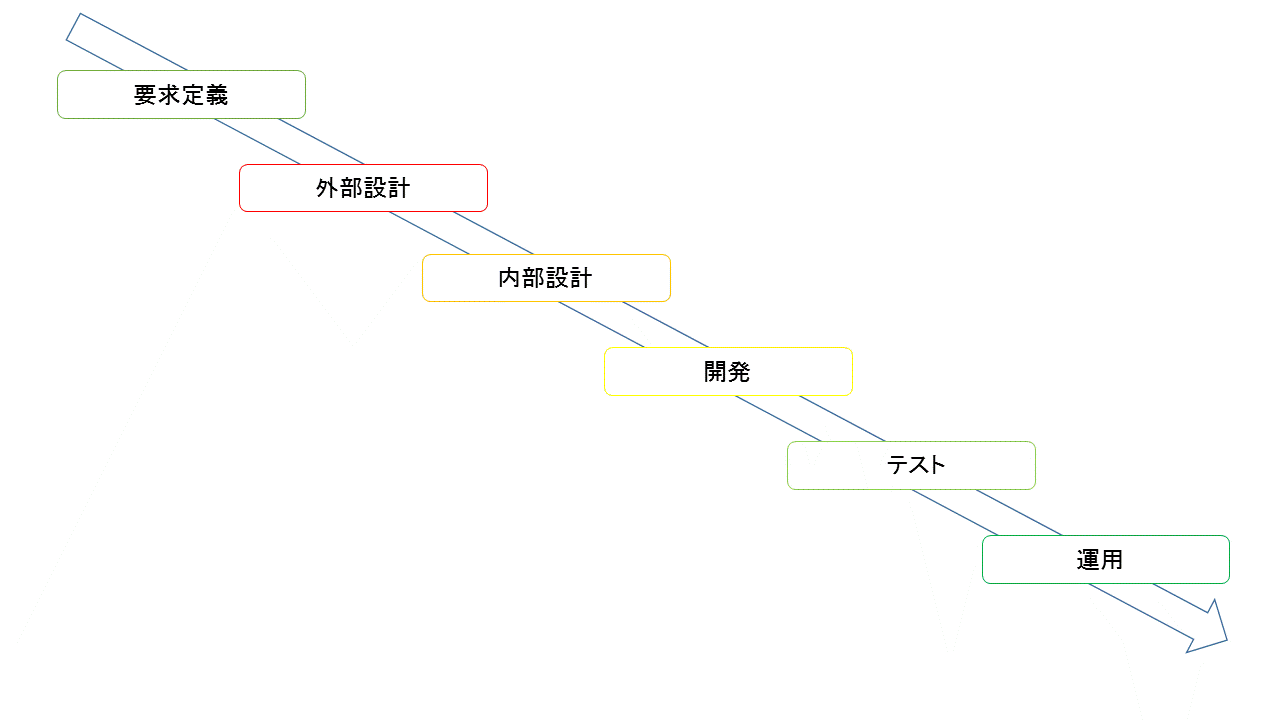
\includegraphics[width=13cm]{waterfall.png}
\caption{ウォーターフォール型開発}
\end{figure}

\newpage

\section{アジャイル型開発}
ソフトウェア開発の手法にアジャイル型開発という開発手法がある.アジャイル型開発は仕様や設計の変更があることを想定し,初めから厳密な仕様や設計は決めない.開発対象を多数の小さな機能に分割し,分割した範囲ごとにおおよその仕様を決める.分割した分,短い期間で実装とテストを繰り返して徐々に開発を進めていくことが出来るので,ウォーターフォール型開発に比べて開発途中の仕様変更が容易でスピードのある開発が可能である.反対に,全体のスケジュールや進捗管理はしにくい\cite{shimizu2012}.

%図の挿入
\begin{figure}[htb]
\centering
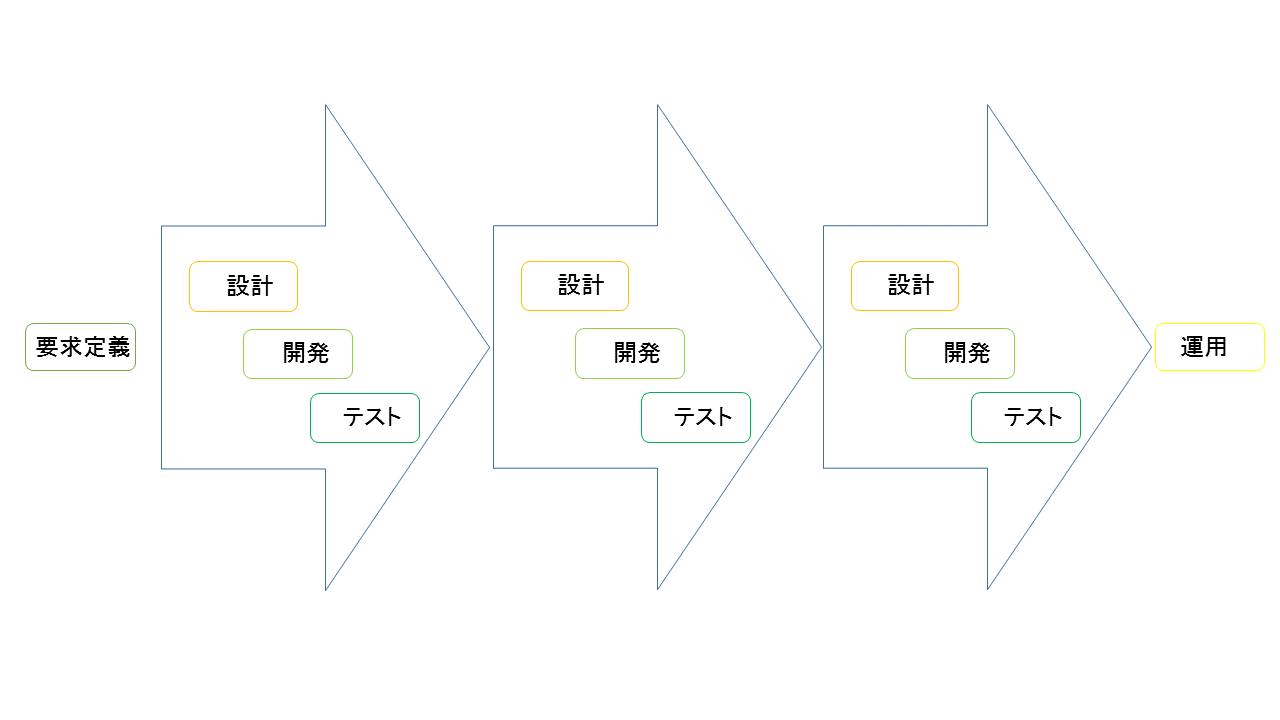
\includegraphics[width=13cm]{agile.png}
\caption{アジャイル型開発}
\end{figure}

\section{開発プロセスの比較}
ウォーターフォール型開発とアジャイル型開発には,それぞれメリットもあればデメリットの面があるため,プロジェクトごとに使い分ける必要がある.銀行システムなど大きくニーズの変化が起きにくいようなプロジェクトでは計画重視のウォーターフォール型開発を採用し,IT市場の進化などに対して柔軟に適応して開発を行う必要があるプロジェクトではアジャイルソフトウェア開発を行う.ソフトウェア開発の現場では,主にウォーターフォール型開発が採用されていたが,現在ではアジャイル型開発が普及してきている.ビジネスにスピードが求められるようになり,システムへの要求事項も刻々と変化するため,ウォーターフォール型開発より市場投入までの期間短縮がしやすいアジャイル型開発が普及してきている\cite{shimizu2012}.

\newpage

\section{テスト駆動開発}
アジャイル型開発では,テスト駆動開発がよく採用される.テスト駆動開発 (Test Driven Development; TDD) とは,プログラム開発手法の一種でプログラムに必要な各機能について最初にテストを書き,そのテストが動作する必要最低限な開発を行った後,コードを洗練させるという短い工程を繰り返し行う手法である.コードをきれいにすることや早い段階で動くコード,フィードバックを確保することが目的に挙げられる.汚いコードや設計が悪いコードは,バグを生みやすくテストもしづらい.テスト駆動開発では,テストと実装を同時に書くことで,そもそもテストしづらいコードが生まれにくくなり,コードが綺麗になる.また,実装の前にテストを書くことで,実装が正しいのかすぐに確かめられる.実装直後はコードの記憶が明確であるので,修正が容易であり,何週間も後にバグのあるコードを読まずに済む\cite{shimizu2012}.

%図の挿入
\begin{figure}[htb]
\centering
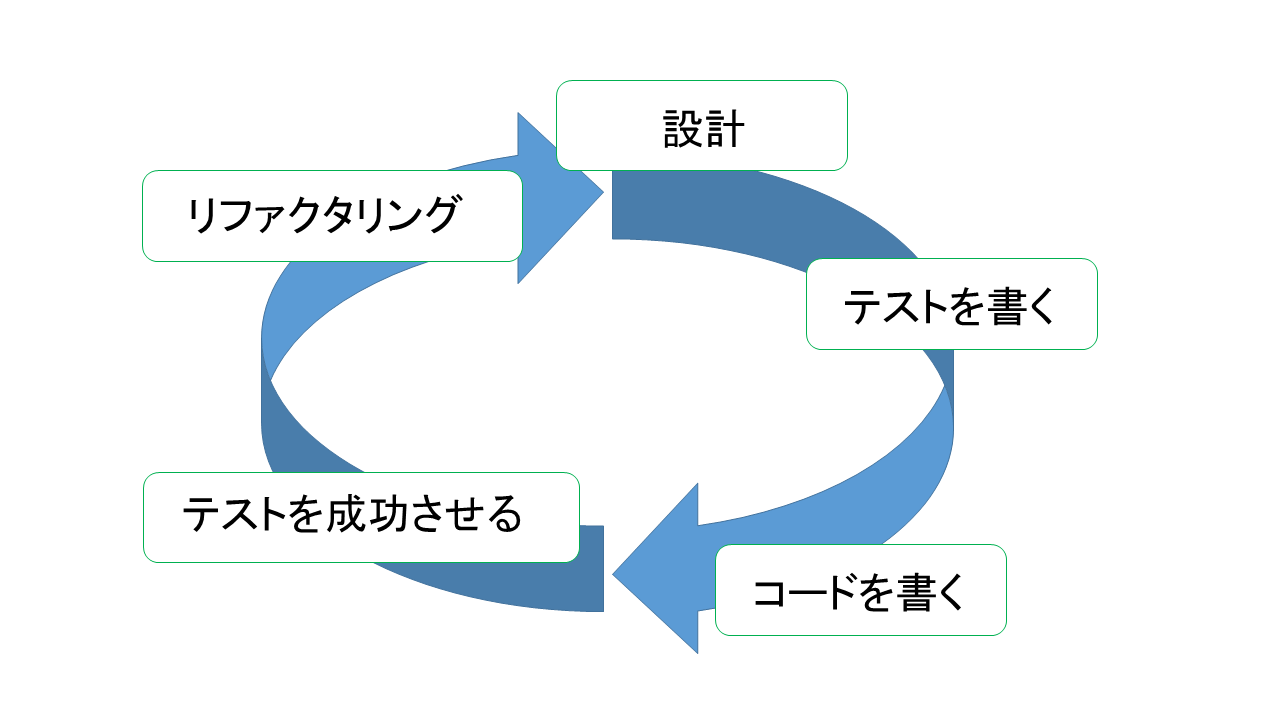
\includegraphics[width=13cm]{tdd.png}
\caption{テスト駆動開発}
\end{figure}

\newpage

\section{オープンソースソフトウェア開発}
開発プロセスに関する情報を誰でも見ることができるオープンソースソフトウェア(OSS)開発というものがある.企業,個人など参加形態を問わずに誰でもプロジェクトに参加することが可能である.

OSS開発には,OSSホスティングサービスを利用して開発されることが多い.オープンソースとは,人間が理解しやすいプログラミング言語で書かれたコンピュータプログラムであるソースコードを広く一般に公開し,誰でも自由に扱ってよいとする考え方である.OSSホスティングサービスとは,そのオープンソースのソフトウェアを格納するリポジトリを中心に,バージョン管理システムや開発者同士の意思疎通の支援,ソフトウェアの公開機能を持つホスティングサーバをインターネット上で提供するサービスである\cite{oss}.

\section{バージョン管理システム}
バージョン管理システムとは,ファイルの作成日時,変更日時,変更点などの履歴を保管することができるシステムである.ソフトウェア開発ではソースコードを作成し,バグの修正や機能の追加ごとにソースコードの状態を記録し,それぞれのバージョンを管理する必要がある.何度も変更を加えたファイルであっても,バージョン管理システムにより,過去の変更内容を確認することや変更前の状態を復元することが容易になる.

多くのバージョン管理システムでは複数の人間がファイルの編集に関わる状況を想定している.複数の人間が複数のファイルをそれぞれ編集すると,ファイルの最新の状態が分からなくなることや同一ファイルに対する変更が競合するなどの問題が生じやすいが,バージョン管理システムではこのような問題を解決できる.

個人のファイル管理に使用することも可能であるし,ソフトウェアのソースコードだけでなく,設定ファイルや原稿の管理などにも使うことも可能である.

バージョン管理システムには,集中型バージョン管理システムと分散型バージョン管理システムがある.

集中型バージョン管理システムは,リポジトリをサーバに集中させて配置するため,1つのリポジトリしか存在しない.データが中央のサーバに集中されるので管理がシンプルであるが,サーバに接続できない状況だと最新のソースコードが取得できないため,開発の進みが遅くなる場合がある.また,サーバが故障等で,最新のソースコードが消えてしまうこともある.

分散型バージョン管理システムは,サーバにある特定のリポジトリを自分のリポジトリに複製し,ローカルで編集できる.サーバにあるリポジトリとは異なるリポジトリとなるため,サーバに接続できなくても開発することができる.分散型は複雑であるが,複数リポジトリがあるのため,編集,やり直しが容易にできる.集中型バージョン管理システムと分散型バージョン管理システムのどちらが良いかは,双方にメリット・デメリットがあるのでケースバイケースである\cite{version}.

\newpage

\section{git}
gitは,プログラムのソースコードなどの変更履歴を記録・追跡するための分散型バージョン管理システムである.Gitのコマンドは様々なものがあるため一部を次に記す.

\hfil
\begin{lstlisting}[basicstyle=\ttfamily\footnotesize, frame=single]
git init
\end{lstlisting}
リポジトリを作成する.

\begin{lstlisting}[basicstyle=\ttfamily\footnotesize, frame=single]
git init –bare
\end{lstlisting}
ベアリポジトリの作成する.

\begin{lstlisting}[basicstyle=\ttfamily\footnotesize, frame=single]
git init –shared
\end{lstlisting}
グループ書き込み権限を有効にする.

\hfil
\begin{lstlisting}[basicstyle=\ttfamily\footnotesize, frame=single]
git clone	
\end{lstlisting}
既存のリポジトリの複製を作成する.

\hfil
\begin{lstlisting}[basicstyle=\ttfamily\footnotesize, frame=single]
git fsck
\end{lstlisting}
リポジトリの正当性チェックする.

\hfil
\begin{lstlisting}[basicstyle=\ttfamily\footnotesize, frame=single]
git gc
\end{lstlisting}
リポジトリ内の不要なオブジェクトを削除し,最適化する.

\hfil
\begin{lstlisting}[basicstyle=\ttfamily\footnotesize, frame=single]
git status
\end{lstlisting}
変更が加えられたファイルを表示する.

\hfil
\begin{lstlisting}[basicstyle=\ttfamily\footnotesize, frame=single]
git diff
\end{lstlisting}
ファイルに加えられた変更点をdiff形式で表示する.

\newpage

\begin{lstlisting}[basicstyle=\ttfamily\footnotesize, frame=single]
git add
\end{lstlisting}
作業ディレクトリ内の変更をステージングエリアに追加する.

\begin{lstlisting}[basicstyle=\ttfamily\footnotesize, frame=single]
git add –a
\end{lstlisting}
すべての変更を含む作業ディレクトリの内容をステージングエリアに追加する.

\begin{lstlisting}[basicstyle=\ttfamily\footnotesize, frame=single]
git add –u
\end{lstlisting}
以前コミットしたファイルだけステージングエリアに追加する.

\hfil
\begin{lstlisting}[basicstyle=\ttfamily\footnotesize, frame=single]
git commit
\end{lstlisting}
ステージングエリアに追加された変更点をコミットする.

\begin{lstlisting}[basicstyle=\ttfamily\footnotesize, frame=single]
git commit -m " <メッセージ> "
\end{lstlisting}
<メッセージ>をコミットメッセージとして,ステージングエリアに追加された変更点をコミットする.

\begin{lstlisting}[basicstyle=\ttfamily\footnotesize, frame=single]
git commit –a
\end{lstlisting}
ステージングエリアに追加されたすべての変更点をコミットする.

\begin{lstlisting}[basicstyle=\ttfamily\footnotesize, frame=single]
git commit –amend
\end{lstlisting}
直前のコミットを修正する.

\hfil
\begin{lstlisting}[basicstyle=\ttfamily\footnotesize, frame=single]
git reset
\end{lstlisting}
直前のコミットを取り消す.

\hfil
\begin{lstlisting}[basicstyle=\ttfamily\footnotesize, frame=single]
git log
\end{lstlisting}
コミットログを表示する.後程詳しい解説をする.

\hfil
\begin{lstlisting}[basicstyle=\ttfamily\footnotesize, frame=single]
git revert
\end{lstlisting}
作業ツリーを指定したコミット時点の状態にまで戻す.

\hfil
\begin{lstlisting}[basicstyle=\ttfamily\footnotesize, frame=single]
git checkout
\end{lstlisting}
ブランチを切り替える.

\newpage

\begin{lstlisting}[basicstyle=\ttfamily\footnotesize, frame=single]
git branch
\end{lstlisting}
ブランチ情報の表示およびブランチの作成する.

\begin{lstlisting}[basicstyle=\ttfamily\footnotesize, frame=single]
git branch –a
\end{lstlisting}
すべてのブランチを確認する.

\begin{lstlisting}[basicstyle=\ttfamily\footnotesize, frame=single]
git branch –r
\end{lstlisting}
リモートブランチを確認する.

\begin{lstlisting}[basicstyle=\ttfamily\footnotesize, frame=single]
git branch –d
\end{lstlisting}
ブランチを削除する.

\hfil
\begin{lstlisting}[basicstyle=\ttfamily\footnotesize, frame=single]
git show-branch
\end{lstlisting}
ブランチの作成,変更,マージ履歴を表示する.

\hfil
\begin{lstlisting}[basicstyle=\ttfamily\footnotesize, frame=single]
git merge
\end{lstlisting}
ローカルブランチをマージする.

\hfil
\begin{lstlisting}[basicstyle=\ttfamily\footnotesize, frame=single]
git tag
\end{lstlisting}
コミットにタグを付ける.

\hfil
\begin{lstlisting}[basicstyle=\ttfamily\footnotesize, frame=single]
git stash
\end{lstlisting}
現在の作業ディレクトリの状態を一時的に保管する.

\hfil
\begin{lstlisting}[basicstyle=\ttfamily\footnotesize, frame=single]
git rebase
\end{lstlisting}
ブランチの派生元を変更する.

\hfil
\begin{lstlisting}[basicstyle=\ttfamily\footnotesize, frame=single]
git pull
\end{lstlisting}
リモートリポジトリの変更点をローカルリポジトリにマージする.

\hfil
\begin{lstlisting}[basicstyle=\ttfamily\footnotesize, frame=single]
git push
\end{lstlisting}
リモートリポジトリに自分のリポジトリの内容を送信する.

\newpage

\begin{lstlisting}[basicstyle=\ttfamily\footnotesize, frame=single]
git remote
\end{lstlisting}
リモートリポジトリの一覧を表示する.

\hfil
\begin{lstlisting}[basicstyle=\ttfamily\footnotesize, frame=single]
git fetch
\end{lstlisting}
リモートリポジトリの最新情報を追加する.

\hfil
\begin{lstlisting}[basicstyle=\ttfamily\footnotesize, frame=single]
git config 
\end{lstlisting}
インストールしたGitに対してコマンドラインから設定を行う.

\hfil
\begin{lstlisting}[basicstyle=\ttfamily\footnotesize, frame=single]
git clean
\end{lstlisting}
作業ディレクトリから追跡対象外のファイルを削除する.

\newpage

\section{GitHub}
よく利用されているOSSホスティングサービスの一つにGitHubがある.GitHubとは,ソフトウェア開発プロジェクトのための共有ウェブサービスであり,アメリカのサンフランシスコを拠点とするGitHub社によって運営されている.GitHubではgitバージョン管理システムを使用し,SNSの機能やプロジェクトのバグ管理に使えるIssues,コードレビューを効率化するPull Requestなどの開発に役立つ機能が多くある.

非公開のリポジトリを作成することもできるため,GitHubを使ってバージョン管理を行っている企業も多数ある.さらに,連携が可能な開発ツールやサービスも多くある.実際,1000万以上のユーザがGitHubを活用しており,リポジトリ数は2430万以上もある.
このように,多くのプロジェクトをホストするGitHubのプロジェクトを調査することにより,ソフトウェア開発の傾向を調べることができると思われる\cite{github}.


\section{GitHubの機能}
GitHubの機能について,一部の説明を次に記す.

\subsection{リポジトリ}
ファイルやディレクトリの状態を記録する場所である.保存された状態は,内容の変更履歴として格納され,変更履歴を管理したいディレクトリをリポジトリの管理下に置くことで,そのディレクトリ内のファイルやディレクトリの変更履歴を記録することができる.

\subsection{リモートリポジトリ}
手元に置いてあるローカルなリポジトリ以外の,ウェブ上に置かれたリポジトリのことである.

\subsection{commit・コミット}
ファイルやディレクトリの追加や変更を,リポジトリに記録するために行う操作のことである.

\subsection{clone・クローン}
サーバにあるリモートリポジトリをローカルにコピーすることである.

\subsection{Push・プッシュ}
リモートリポジトリに自分の変更履歴がアップロードされて,リモートリポジトリ内の変更履歴がローカルリポジトリの変更履歴と同じ状態にすることである.

\newpage

\subsection{branch・ブランチ}
履歴の流れを分岐して記録するためのものである.分岐したブランチは他のブランチの影響を受けないため,同じリポジトリ中で複数の変更を同時に進めていくことができる.

\subsection{pull・プル}
リモートリポジトリから最新の変更履歴をダウンロードしてきて,自分のローカルリポジトリにその内容を取り込むことである.

\subsection{Pull Request・プルリクエスト}
相手に対して自分のブランチをpullしてもらうように要求する機能のことである.

\subsection{Origin}
clone元のリモートリポジトリのことである.

\subsection{ステージング}
修正作業によって更新したもののうち,コミット対象の更新を選り分けるための作業のことである.

\subsection{ステージングエリア}
ステージングを行う領域のことである.

\subsection{Revert}
ステージングエリアに追加した変更を戻すことである.

\subsection{タグ}
コミットを参照しやすくするために,わかりやすい名前を付けるものである.

\subsection{ラベル}
自由に作成でき,Issueをフィルタリングできる機能である.

\newpage

\subsection{チェックアウト}
ブランチ内から作業ディレクトリに展開されたファイル・ディレクトリ群のことである.

\subsection{トラック}
Git上で変更内容を追跡できるようにすることである.特に,ローカルブランチとリモートブランチとを紐付けすることである.また,ファイルやディレクトリに対して言う場合は,Gitオブジェクトに変換してリポジトリに格納することである.

\subsection{作業ツリー}
ブランチ内から作業ディレクトリに展開されたファイル・ディレクトリ郡のことである.

\subsection{Merge・マージ}
当該ブランチに対して別のブランチの差分を取り込むことである.

\subsection{リベース}
マージの一種で,当該ブランチの更新差分を無かったことにして,別ブランチの最新を取り込んだ後,当該ブランチの更新差分を適用する処理することである.

\subsection{チェリーピック}
マージの一種で,全ての差分を取り込むのではなく,特定のコミットを指定して取り込むことである.

\subsection{競合}
マージの際に,同一のファイル・ディレクトリに対しての更新が発生していることである.

\subsection{fech・フェッチ}
リモートリポジトリの最新を取り込むことである.

\subsection{Fork・フォーク}
GitHubのサービスで,相手のリポジトリを自分のリポジトリとしてコピー・保持できる機能のことである.

\newpage

\subsection{Issue}
一つのタスクを一つのIssueに割り当てて,トラッキングや管理を行えるようにするための機能である.

\subsection{Wiki}
Wiki機能は,いつでもだれでも文書を書き換えて保存できるため,共同で文章を作成できる機能である.

\subsection{MileStone・マイルストーン}
やるべきタスクの管理にIssueを用いることができるようにする機能である.

\subsection{Gist}
コードの断片など,リポジトリに入れるほどでもないコードを管理,公開するのに重宝する機能である.また,ブログなどを書いている人はGistにサンプルコードを登録すれば,ブログの記事に埋め込むこともできる.

\subsection{News Feed}
フォローしているユーザやWatchしているプロジェクトの活動情報が流れてくる機能である.最新の動向を確認することである.

\subsection{スター}
GitHub内のプロジェクトをお気に入りできる機能である.

\subsection{リビジョン}
ある期間内までの過去のプロジェクトデータやある程度まとまったプロジェクトデータを記録したものである.

\newpage

\section{パレートの法則}
パレートの法則とは,経済において,全体の数値の大部分は全体を構成するうちの一部の要素が生み出しているという理論である.80:20の法則,ばらつきの法則とも呼ばれる.パレートの法則は経済以外にも,自然現象や社会現象などさまざまな事例に当て嵌められることが多い.ただし,現代で言われるパレートの法則の多くは,法則と言うよりも経験則の類である\cite{pare}.

パレートの法則が用いられる事象の例を次に挙げる.
\begin{itemize}
\item ビジネスにおいて,売上の80\%は全顧客の20\%が生み出している.よって売上を伸ばすには顧客全員を対象としたサービスを行うよりも,20\%の顧客に的を絞ったサービスを行う方が効率的である.
\item 商品の売上の80\%は全商品銘柄のうちの20\%で生み出している.
\item 売上の80\%は全従業員のうちの20\%で生み出している.
\item 仕事の成果の80\%は費やした時間全体のうちの20\%の時間で生み出している.
\item プログラムの処理にかかる時間の80\%はコード全体の20\%の部分が占める.
\end{itemize}



\chapter{目的}	
本研究では,GitHub上のプロジェクトを調査する.テスト駆動開発において,個人の貢献度がメインコードとテストコードで違いがあるのかを調査する.


\chapter{手法}
以下の手順で研究を進める.
\begin{enumerate}
\item GitHubのプロジェクトでテストコードがあるプロジェクトを探す.
\item プロジェクトのコミットごとにユーザ名,日時,メインコードの行数,テストコードの行数をそれぞれ取得できるプログラムを作成する.
\item 作成したプログラムを実行する.
\item 取得したデータをメンバごとにソートし,メインコードとテストコードの行数を集計する.
\item メンバごとの行数を比較し,パレートの法則が成り立つか調査をする.\end{enumerate}

\section{調査対象のプロジェクト}
GitHubのプロジェクトでテストコードがあるプロジェクトを探す.GitHubでホスティングされているプロジェクトを無作為に抽出(ランダムサンプリング)を行い,testフォルダがある場合にそのプロジェクトを調査の対象とする.

\newpage

本研究で調査するプロジェクトを次に記す.

\begin{table}[h]
 \begin{center}
 \caption{調査対象プロジェクト}
  \begin{tabular}{|l|l|} \hline
    ユーザ名 & リポジトリ名\\ \hline
    angular & angular.js\\ \hline
    caolan & async\\ \hline
    jashkenas & backbone\\ \hline
    bower & bower\\ \hline
    adobe & brackets\\ \hline
    jashkenas & coffee-script\\ \hline
    Shopify & dashing\\ \hline
    plataformatec & devise\\ \hline
    discourse & discourse\\ \hline
    visionmedia & express\\ \hline
    gruntjs & grunt\\ \hline
    visionmedia & jade\\ \hline
    jekyll & jekyll\\ \hline
    jquery & jquery\\ \hline
    less & less.js\\ \hline
    janl & mustache.js\\ \hline
    mozilla & pdf.js\\ \hline
    scottjehl & Respond\\ \hline
    resque & resque\\ \hline
    hakimel & reveal.js\\ \hline
    LearnBoost & socket.io\\ \hline
    jashkenas & underscore\\ \hline
  \end{tabular}
  \label{tab:project}
  \end{center}
\end{table}

\newpage

\section{プログラムの作成}
調査対象のプロジェクトからデータを取得するプログラム作成する.作成するプログラムでは,プロジェクトのコミットごとにユーザ名,日時,メインコードの行数,テストコードの行数をそれぞれ取得できるようにする.

作成下プログラムは次の2つか成り立つ.

lineCounter.sh
\begin{lstlisting}[basicstyle=\ttfamily\footnotesize, frame=single]
#!bin/bash
cd $1
git log --pretty=format:"%H,%cn,%cd" --date=iso --first-parent --no-merges >
 ../$1-commits.csv
cd ..
cat $1-commits.csv | python lineCountScriptCreator.py $1 > $1-count.sh
bash $1-count.sh > $1-count-result.csv 2> $1-error.log
awk -F ',' 'BEGIN{OFS=","} {print $0,$4-$5;}' $1-count-result.csv >
 $1-result.csv
\end{lstlisting}

\hfil
lineCountScriptCreator.py
\begin{lstlisting}[basicstyle=\ttfamily\footnotesize, frame=single]
from datetime import datetime
from dateutil.parser import parse
from dateutil import tz
import sys
myProject = sys.argv[1].replace("'", "\\'")
print("rm %s-error.log") % (myProject)
for line in sys.stdin:
  x = line.split(',')
  myHash = x[0]
  myName = x[1]
  myDate = datetime.strftime(parse(x[2]).astimezone(tz.gettz('UTC')),
 '%Y-%m-%d %H:%M:%S')
  print("echo %s >&2") % (myHash)
  print("cd %s") % (myProject)
  print("git checkout -f %s 2>> ../%s-checkout-error.log") %
 (myHash, myProject)
  print("cd ..")
  print("if [ -e %s/test ]; then") % (myProject)
  print(" echo %s,%s,%s,$(grep -rI '' '%s' | grep -v '^%s/\.git/' | wc -l),
 $(grep -rI '' '%s/test' | wc -l)") % (myHash, myName, myDate, myProject,
 myProject, myProject)
  print("else")
  print(" echo %s,%s,%s,$(grep -rI '' '%s' | grep -v '^%s/\.git/' | wc -l),0") 
 % (myHash, myName, myDate, myProject, myProject)
  print("fi")
\end{lstlisting}

\newpage

\subsection{lineCounter.shの解説}
\begin{lstlisting}[basicstyle=\ttfamily\footnotesize, frame=single]
#!bin/bash
\end{lstlisting}
先頭に指定した「\#!」で始まる「シバン」と呼ばれる文字列は,スクリプトを実行するためのインタプリタを指定する.「このシェルスクリプトはbashによって解釈,実行される」と宣言するためのものである.これは決まり文句のようなもので,必ず1行目に指定する.

\hfil
\begin{lstlisting}[basicstyle=\ttfamily\footnotesize, frame=single]
cd <パス>
\end{lstlisting}
「cd」とは,指定したディレクトリに移動することができるコマンドである.<パス>には現在位置から,目的のファイルやフォルダまでの道筋である相対パスと最上位階層から目的のファイルやフォルダまでのすべての道筋である絶対パスのどちらでも使用できる.

次の記号を使うことによって,ディレクトリを移動することもできる.

{
\small
\begin{verbatim}
cd /
\end{verbatim}
}
ルート・ディレクトリ(システム上最上層のディレクトリ)に移動する.

{
\small
\begin{verbatim}
cd ..
\end{verbatim}
}
親ディレクトリ(一階層上のディレクトリ)に移動する.

{
\small
\begin{verbatim}
cd ~/
\end{verbatim}
}
ホームディレクトリ(ユーザ上最上層ディレクトリ)に移動する.

\hfil
\begin{lstlisting}[basicstyle=\ttfamily\footnotesize, frame=single]
git log <オプション>
\end{lstlisting}
「git log」とはリポジトリの履歴情報を見るコマンドである.デフォルトでは直近のコミットしか見られないため,オプションを使うことによってさまざまな履歴情報を見ることができる.また,最後に「 > “ファイル名”」と入れることによって,ファイルに情報を書き出すことができる.

オプションを次に記す.

{
\small
\begin{verbatim}
-p -<表示する数>
\end{verbatim}
}
各コミットのパッチを表示する.

{
\small
\begin{verbatim}
--word-diff
\end{verbatim}
}
変更点を単語単位で表示する.

{
\small
\begin{verbatim}
--stat
\end{verbatim}
}
各コミットで変更されたファイルの統計情報を表示する.

{
\small
\begin{verbatim}
--first-parent
\end{verbatim}
}
ブランチを指定する.

{
\small
\begin{verbatim}
--abbrev-commit
\end{verbatim}
}
SHA-1 チェックサムの全体ではなく最初の数文字のみを表示する.

{
\small
\begin{verbatim}
--name-only
\end{verbatim}
}
コミット情報の後に変更されたファイルの一覧を表示する.

{
\small
\begin{verbatim}
--relative-date
\end{verbatim}
}
完全な日付フォーマットではなく,相対フォーマットで日付を表示する.

{
\small
\begin{verbatim}
--no-merges
\end{verbatim}
}
マージコミットを除外する.

{
\small
\begin{verbatim}
--grep <単語>
\end{verbatim}
}
検索をする.

{
\small
\begin{verbatim}
--pretty=format:"<オプション記号>"
\end{verbatim}
}
コミットを別のフォーマットで表示する.
\begin{table}[hbtp]
\caption{オプション記号}
\label{table:data_type}
\centering
\begin{tabular}{lcr}
\hline
記号 & 説明 \\
\hline
\hline
\%H & コミットのハッシュ \\
\%h & コミットの短縮ハッシュ \\
\%T & ツリーのハッシュ \\
\%t & ツリーの短縮ハッシュ \\
\%P & 親のハッシュ \\
\%p & 親の短縮ハッシュ \\
\%an & Authorの名前 \\
\%ae & Authorのメールアドレス \\
\%ad & Authorの日付 \\
\%ar & Authorの相対日付 \\
\%cn & Committerの名前 \\
\%ce & Committerのアドレス \\
\%cd & Committerの日付 \\
\%cr & Committerの相対日付 \\
\%s & 件名 \\
\hline
\end{tabular}
\end{table}

\newpage

\begin{lstlisting}[basicstyle=\ttfamily\footnotesize, frame=single]
cat <ファイル名.csv> | python lineCountScriptCreator.py <リポジトリ名>
 > <ファイル名.sh>
\end{lstlisting}
「cat」とは,ファイルまたは標準入力の内容をそのまま標準出力に出力するコマンドである.ファイルの中身を確認することができる.また,複数のファイルを指定することで,複数のファイルを連結するのに使うことができる.「\textbar(パイプ)」とは,コマンドの標準出力を次のコマンドに渡す処理ができるコマンドである.「cat」で開いた内容を「lineCountScriptCreator.py」に渡す.lineCountScriptCreator.pyはgitの履歴情報からソースコードの行数をカウントするスクリプトを作成するプログラムである.lineCountScriptCreator.pyについては後程説明をする.

\hfil
\begin{lstlisting}[basicstyle=\ttfamily\footnotesize, frame=single]
bash <リポジトリ名.sh> > <リポジトリ名.csv> 2 > <ファイル名-error.log>
\end{lstlisting}
「bash」とは,ユーザによってキーボードから入力された文字やマウスのクリックなど,与えられた指示をOSの中核部分に伝え,対応した機能を実行するようにOSに指示を伝えるコマンドである.lineCountScriptCreator.pyにて作成されたスクリプトの実行とその結果をCSV形式に書き出し,エラーがあればエラーログに書き出す.

\hfil
\begin{lstlisting}[basicstyle=\ttfamily\footnotesize, frame=single]
awk -F ',' 'BEGIN{OFS=","} {print $0,$4-$5;}' <ファイル名_tmp.csv> >
 <ファイル名.csv>
\end{lstlisting}
「awk」とは,区切られた複数列のテキストデータを処理するときに使うコマンドである.四則演算などもでき,渡されたファイルの一行ずつを処理する.上記の例だと,「-F」はCSV形式の区切りの文字列を表す.「BEGIN」は読み込み開始とともに実行するという意味である.「OFS」は出力時の区切りを設定する.printは出力する内容を表す.print内で「\$0」というのは元のデータをそのまま出力するという意味である.また,「\$4-\$5」というのは「4列目-5列目(コード合計-テストコード)」を表す.前者のファイル名には整理したファイル名,後者には整理後の保存したいファイル名を入力する.

\newpage

\subsection{lineCountScriptCreator.pyの解説}
\begin{lstlisting}[basicstyle=\ttfamily\footnotesize, frame=single]
from datetime import datetime
from dateutil.parser import parse
from dateutil import tz
import sys
\end{lstlisting}
「from import」で指定したモジュールをインポートができる.

\hfil
\begin{lstlisting}[basicstyle=\ttfamily\footnotesize, frame=single]
myProject = sys.argv[1].replace("'", "\\'")
\end{lstlisting}
渡された引数(今回はリポジトリ名)を「 ' 」から「\verb|\|\verb|\|'」に置換してmyProject変数に保存する.

\hfil
\begin{lstlisting}[basicstyle=\ttfamily\footnotesize, frame=single]
print("rm %s-error.log") % (myProject)
\end{lstlisting}
“リポジトリ名”-error.logの削除を行う.

\hfil
\begin{lstlisting}[basicstyle=\ttfamily\footnotesize, frame=single]
for line in sys.stdin:
\end{lstlisting}
読み込んだファイルの一行一行を処理して繰り返す.

\hfil
\begin{lstlisting}[basicstyle=\ttfamily\footnotesize, frame=single]
x = line.split(',')
\end{lstlisting}
CSV形式には「Hash,Name,Date」と別れているので「 , 」xに配列を使って変数として入れる.

\hfil
\begin{lstlisting}[basicstyle=\ttfamily\footnotesize, frame=single]
myHash = x[0]
\end{lstlisting}
MyHash変数にx[0]を代入する.つまり,MyHash変数にはHashが代入される.

\hfil
\begin{lstlisting}[basicstyle=\ttfamily\footnotesize, frame=single]
myName = x[1]
\end{lstlisting}
MyName変数にx[1]を代入する.つまり,MyName変数にはNameが代入される.

\hfil
\begin{lstlisting}[basicstyle=\ttfamily\footnotesize, frame=single]
myDate = datetime.strftime(parse(x[2]).astimezone(tz.gettz('UTC')),
 '%Y-%m-%d %H:%M:%S')
\end{lstlisting}
myDate変数にx[2]を代入している代入する.つまり,MyDate変数にはDateが代入される.また,git logで取得したデータの時間は投稿した人の国のタイムゾーンが記載されているので全てをUTC(協定世界時)に変換する.

例)2017-01-10 00:38:56 -0500 → 2017-01-10 05:38:56

\hfil
\begin{lstlisting}[basicstyle=\ttfamily\footnotesize, frame=single]
print("echo %s >&2") % (myHash)
print("cd %s") % (myProject)
print("git checkout -f %s 2>> ../%s-checkout-error.log") % (myHash, myProject)
print("cd ..")
\end{lstlisting}
エラーログを出力する.

\hfil
\begin{lstlisting}[basicstyle=\ttfamily\footnotesize, frame=single]
print("if [ -e %s/test ]; then") % (myProject)
print(" echo %s,%s,%s,$(grep -rI '' '%s' | grep -v '^%s/\.git/' | wc -l),
 $(grep -rI '' '%s/test' | wc -l)") % (myHash, myName, myDate,
 myProject, myProject, myProject)
print("else")
print(" echo %s,%s,%s,$(grep -rI '' '%s' | grep -v '^%s/\.git/' | wc -l),0")
 % (myHash, myName, myDate, myProject, myProject)
print("fi")
\end{lstlisting}
IF[条件式]…Aの処理…else…Bの処理という構文である.

条件式はリポジトリにtestディレクトリの中にフォルダがあるかないかを判別する.testディレクトの中にファイルがある場合はAの処理を行う.testディレクトの中にファイルがない場合はBの処理を行う.Aでは,Hash,Name,Date,.gitフォルダ(履歴情報)を除いた行数とtestディレクトリの行数を出力という処理を行う.Aの処理だけでは,testディレクトリの中にファイルがない場合にエラーが出てしまい,正常にカウントできないので,Bの処理を行う.Bの処理では,testディレクトリの行数を0と出力する.

\newpage

\section{プログラムの実行}
プログラムの実行環境はLinuxを想定する.今回はLinuxディストリビューションの一種であるCentOS7を使用する.用意したコンピュータのOSはWindowsのため,VirtualBoxとVagrantを使用して仮想マシンを作成し,CentOS7を導入する.また,必要なソフトウェアを簡単に導入,管理するためにChocolateyをインストールする.

%図の挿入
\begin{figure}[h]
\centering
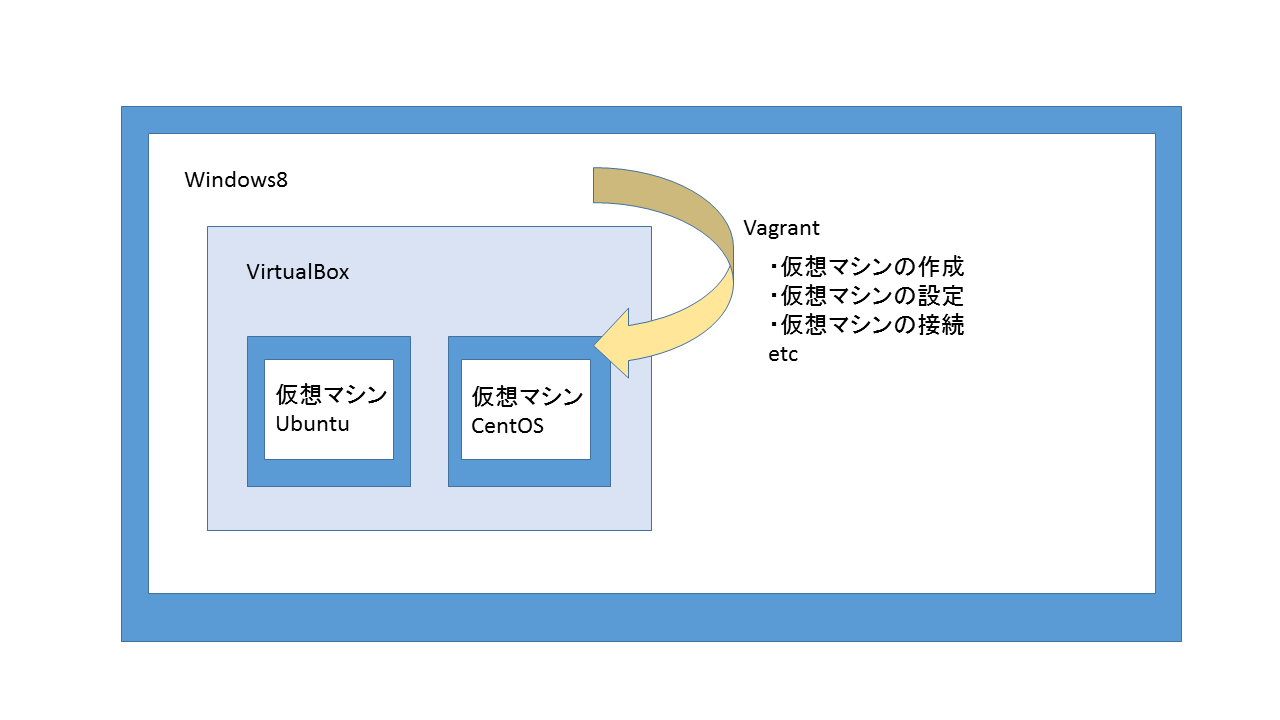
\includegraphics[width=13cm]{kankyou.png}
\caption{実行環境}
\end{figure}

\newpage

\subsection{Linuxとは}
Linuxとは,狭義ではLinuxカーネル,広義ではそれをカーネルとして用いたシステムを指すUnix系オペレーティングシステムである.

Linuxは,スーパーコンピュータ,メインフレーム,サーバ,パーソナルコンピュータ,組み込みシステム,幅広い種類のハードウェアと共に使用されている.特にサーバ,メインフレーム,スーパーコンピュータ用のOSとして使用される.携帯電話,ネットワークルータ,テレビ,ハードディスクレコーダ,カーナビゲーションシステムといった組み込みシステムでもよく使われている.スマートフォンやタブレット端末用プラットフォームAndroidはLinuxカーネルの上に構築されている.

Linuxの開発は,フリーかつオープンソースなソフトウェアの共同開発として最も傑出した例のひとつである.Linuxカーネルのソースコードは無償で入手でき,GNU一般公衆利用許諾書のもとにおいて,非営利・営利に関わらず誰でも自由に使用,修正,頒布できる.Linuxは,世界中の開発者の知識を取り入れるという方法によって,あらゆる方面に利用できる幅広い機能と柔軟性を獲得し,数多くのユーザの協力によって問題を修正していくことで高い信頼性を獲得した.

デスクトップやサーバ用のLinuxは,Linuxディストリビューションという形でパッケージ化され配布されている.有名なLinuxディストリビューションとしては,Debianとその派生であるUbuntu,Linux MintやRed Hat Linuxとその派生であるFedora,Red Hat Enterprise Linux,CentOSなどがある.各Linuxディストリビューションは,Linuxカーネル,システムソフトウェア,ライブラリ等,巨大なコンパイル済のアプリケーション群を含んでいる.

デスクトップOSとしてLinuxを使用することは,かつては技術者や上級ユーザだけが行うことというイメージが強かったが,最近では一般ユーザでも容易に使用できる.デスクトップ環境が充実したり,非常に簡単にインストールできるディストリビューションが登場したり,各種ハードウェアへの対応や自動設定機能が大幅に向上するなどしたためである.サーバでの利用を想定したディストリビューションなどでは,標準インストールからグラフィカルインタフェースをすべて排除しているものもある.また,Linuxは自由に再頒布できるので,独自のディストリビューションを作ることも自由である\cite{linux}.

\newpage

\subsection{CentOSとは}
CentOSとは,商用Linuxディストリビューション「Red Hat Enterprise Linux」との完全互換を目指したオープンソースLinuxディストリビューションである.CentOSという名前は,「Community Enterprise Operating System」コミュニティベースで開発されたエンタープライズレベルのOSの略表記と言われている.Linuxディストリビューションの代表格となっており,CentOSプロジェクトによって,積極的にオープンな開発が行われている.

CentOSは,「Red Hat Enterprise Linux」の中のフリーライセンスで使えるパーツを組み合わせた形でリビルドされている.そのため,ライセンス費用がゼロで導入コストを節減できる.商用製品である「Red Hat Enterprise Linux」とほぼ同等の機能を持ち,さまざまな用途に対応できるサーバOSとして,高い品質を備え,長期間運用に耐えうる安定性がある.

CentOSはサーバでの長期間稼働を想定し,安定性を優先した設計思想になっている.最新技術を頻繁に取り込んでいくようなことがないため,他のOSやディストリビューションに比べて,アップデートの回数が少なめになっている.サーバOSにとって,アップデートのためにサーバを停止させる回数が少ないというのは,重要なポイントである.

オフィススイートやマルチメディアツールなどのインストールをして環境設定をすることによって,デスクトップOSとして使用できる.CentOSは有償のOSを使いつつ,無償での提供を実現した優秀なOSであることやサーバで非常に役に立つことから,Linuxでの環境を構築するには最適である\cite{centos}.

\newpage

\subsection{VirtualBoxとは}
VirtualBoxとは,オープンソースの仮想化ソフトウェアの一つである.現在の開発は米国オラクルが行っている.既存のオペレーティングシステム(ホストOS)上にアプリケーションの一つとしてインストールされ,その中で追加のオペレーティングシステム(ゲストOS)を実行することができる.例えば,Windows8がホストOSとして動作しているマシン上で,CentOSをゲストOSとすることができる.サポートされるホストOSはLinux,macOS,Microsoft Windows,Solarisである.また後述するように,ソースコードが配布されているため,他のUnix系のOSでも導入できる.例えば,FreeBSDではportsで導入することができる.ゲストOSとしてサポートされるのは,FreeBSD,Linux,OpenBSD,OS/2 Warp,Windows,Mac OS X Server,Solarisなど多岐にわたる.x86/x64アーキテクチャのOSであれば基本的に動作する\cite{vbox}.

VirtualBox本体により提供される基本機能の一部を次に記す.
\begin{itemize}
\item スナップショット
\item シームレスモード
\item クリップボード
\item 共有フォルダ
\item シリアルデバイスとシステム間の切替えを支援するユーティリティ
\item コマンドラインからの操作
\item リモートディスプレイ
\end{itemize}

\newpage

\subsection{Vagrantとは}
Vagrantとは,仮想開発環境構築ソフトウェアである.Vagrantを用いると,構成情報を記述した設定ファイルを元に,仮想環境の構築から設定までを自動的に行うことができる.以前はVirtualBoxをターゲットとしていたが,1.1以降のバージョンではVMwareなどの他の仮想化ソフトウェアやAmazon EC2のようなサーバ環境も対象とできるようになった.Vagrant自身はRubyで作成されているが,PHPやPython,Java,C\#,JavaScriptといった他のプログラミング言語の開発においても用いることができる.VagrantはChef,puppetなどの構成管理ツールと連携して環境構築を自動化できる.開発環境を構築する際,通常は環境構築手順書を見ながら開発者が自分のローカル環境に構築するが,環境構築を自動化してしまえば環境構築する手間と環境構築手順書を書く手間を省ける.ネットワーク上にあるBoxファイルを共有することが容易なのでチームで同一の環境を構築することが簡単にできる\cite{vagrant}.

vagrantのコマンドを次に記す.

{
\small
\begin{verbatim}
vagrant up
\end{verbatim}
}
Vagrantfileに記述された設定を読み込み,仮想マシンを起動する.

{
\small
\begin{verbatim}
vagrant halt
\end{verbatim}
}
起動しているvagrantを停止する.

{
\small
\begin{verbatim}
vagrant reload
\end{verbatim}
}
起動している仮想マシンを再起動する.

{
\small
\begin{verbatim}
vagrant desutroy
\end{verbatim}
}
仮想マシンを消去する.

{
\small
\begin{verbatim}
vagrant status
\end{verbatim}
}
仮想マシンの状態を確認する.

\subsection{Chocolateyとは}
Chocolateyとは,Windows上で動作するソフトウェアをコマンドラインからインストール,アンインストール,アップデート,検索することができるパッケー管理ツールである.有名なソフトウェアはだいたいChocolateyで入れることができる.ブラウザから公式サイトにアクセスし,ダウンロード,インストールという手順を踏まずに,コマンドラインから1発でインストールできる手軽さは非常に魅力的である.

\newpage

\subsection{実行環境の準備}
\subsection{Chocolateyのインストール}
Chocolateyのインストールを行う.Chocolateyのインストールは,Chocolateyのサイト(https://chocolatey.org/install)に掲載されているコマンドを実行すればできる.

%図の挿入
\begin{figure}[h]
\centering
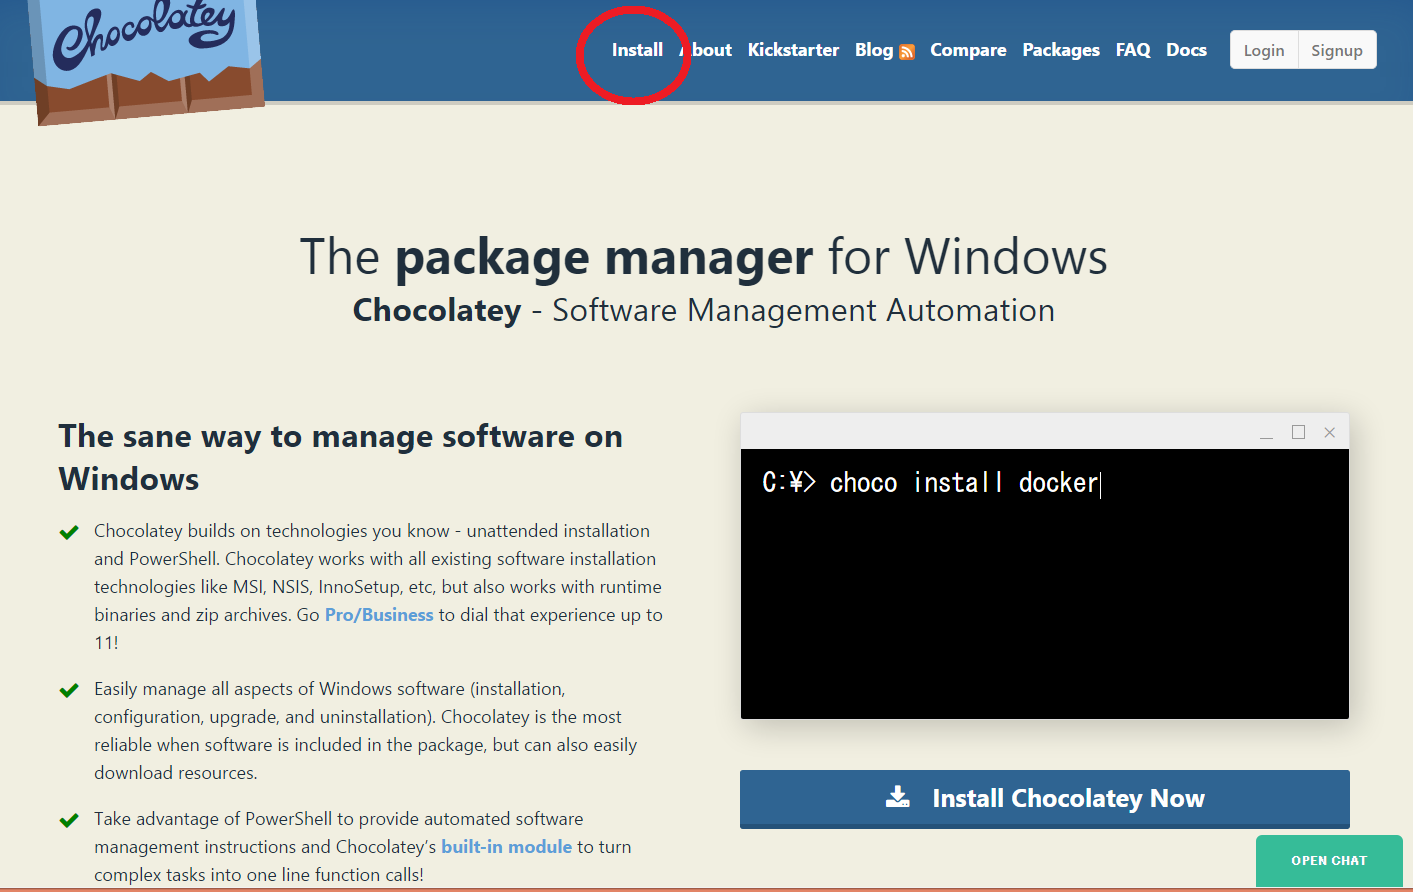
\includegraphics[width=11cm]{choco1.png}
\caption{Chocolateyの公式サイト}
\end{figure}

Chocolateyのサイトに下記の画像ようなページがあるので,赤丸と同じ部分をダブルクリックする.コマンドがコピーされるので,管理者のコマンドプロンプトに貼り付けてEnterキーを押せば実行される.

%図の挿入
\begin{figure}[h]
\centering
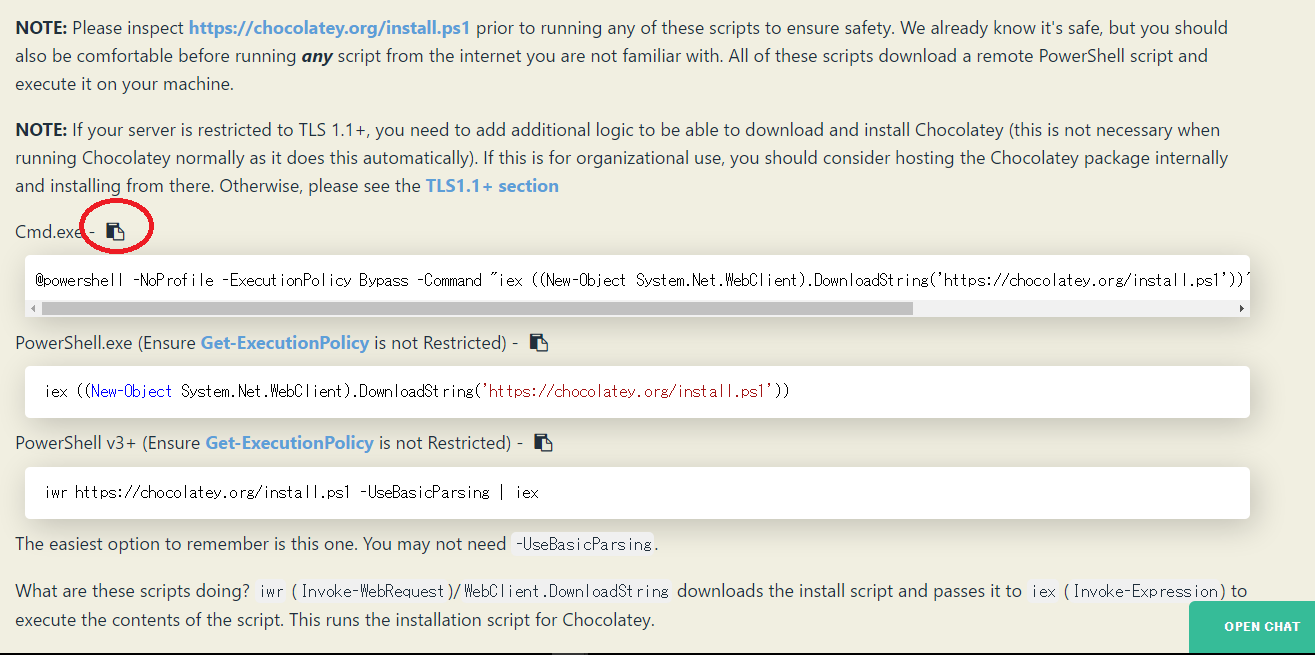
\includegraphics[width=11cm]{choco2.png}
\caption{Chocolateyの公式サイト-インストールページ}
\end{figure}

\newpage

\subsection{VirtualBoxとVagrant}
導入したChocolateyでVirtualBoxとVagrantをインストールする.インストール方法は管理者のコマンドプロンプトを開いてchocolatey installコマンドを使用するだけである.このコマンドはcinstと省略できる.バージョンについては,特に気になければChocolateyのライブラリにある最新パッケージが適用される.
以下のコマンドでインストールする.
\begin{lstlisting}[basicstyle=\ttfamily\footnotesize, frame=single]
cinst virtualbox
cinst vagrant
\end{lstlisting}

\subsection{仮想マシンの作成}
仮想マシンを作成し,CentOS7を導入する.今回はmyVagrantフォルダ作成し,以下で作業を行う.

\begin{lstlisting}[basicstyle=\ttfamily\footnotesize, frame=single]
cd myVagrant
mkdir myCentos
cd myCentos
vagrant init puphpet/centos7-x64
vagrant up
\end{lstlisting}
\hfil

以上で仮想マシンの準備は完了である.

\subsection{仮想マシンの接続}
ゲストOSに接続する.接続には以下のコマンドを使用する.
\begin{lstlisting}[basicstyle=\ttfamily\footnotesize, frame=single]
vagrat ssh
\end{lstlisting}

ユーザ:vagrant,パスワード:vagrantでログインすることができる.

\subsection{共有フォルダの作成}
ホストOSとゲストOSで共有のフォルダを作成する.デバイス→共有フォルダで共有したいホストのフォルダを選択する.ここではDesktopとする.ゲストOSのコンソールでmkdir shareなどとして共有用のフォルダを作成する.

以下のコマンドでフォルダを共有する.
\begin{lstlisting}[basicstyle=\ttfamily\footnotesize, frame=single]
sudo mount -t vboxsf Desktop share
\end{lstlisting}
\hfil

以上でゲストOSのshareがホストOSのDesktopと同じになる.

\newpage

\subsection{コマンドのインストール}
必要なコマンドのインストールを行う.

gitのインストール
GitHubのプロジェクトからデータを取得するため,gitをインストールする.git clone等のコマンドが使用できるようになる.
\begin{lstlisting}[basicstyle=\ttfamily\footnotesize, frame=single]
sudo yum install –y git
\end{lstlisting}
\hfil

dateutilのインストール
作成したプログラムでPythonのライブラリのdateutil.parserを使用しているので, dateutilをインストールする.dateutil.parserを使うと,日付を表す文字をdatetimeオブジェクトに変換できる.
\begin{lstlisting}[basicstyle=\ttfamily\footnotesize, frame=single]
sudo yum install -y python-dateutil
\end{lstlisting}


\section{プログラムの実行}

\subsection{リポジトリのクローン}
調査するプロジェクトのリポジトリをクローンする.
git clone <URL>でGitHub上のプロジェクトをクローンすることができる.「git clone」とは,リポジトリを複製(ローカル環境へコピー)するためのコマンドである.オプション指定をすることによって,次のようなことができる.

{
\small
\begin{verbatim}
git clone <URL> <ディレクリ名>
\end{verbatim}
}
ディレクトリ名の指定をする.

{
\small
\begin{verbatim}
git clone –depth 1 <URL>
\end{verbatim}
}
新リビジョンのみの取得をする.

\hfil
※git cloneはリポジトリの履歴情報までも含めてリポジトリを複製するため,大規模なプロジェクトの場合は多くのファイルを取得・コピーしなければならないことがある.最新のソースファイルを取得する目的のみで使用する場合は,「--depth」オプションで取得するとよい.

プロジェクトをクローンすることができたら,以下のコマンドでプログラムを実行する.
\begin{lstlisting}[basicstyle=\ttfamily\footnotesize, frame=single]
bash lineCounter.sh <リポジトリ>
\end{lstlisting}
\hfil

リポジトリ名-result.csvのファイルにコミットID,名前,日時,プロジェクト全体のコード行数,テストコードの行数,メインコードの行数が取得されているはずである.

\newpage

取得したデータをメンバごとにソートし,メインコードとテストコードの行数を集計する.

データの取得ができていれば,ファイル名を<リポジトリ>-result.xlsxにエクスポート(csv形式からスプレットシート形式に変換)し,データを処理する.図1の1行目のように作業が行いやすくなるような見出しを追加する.

%図の挿入
\begin{figure}[h]
\centering
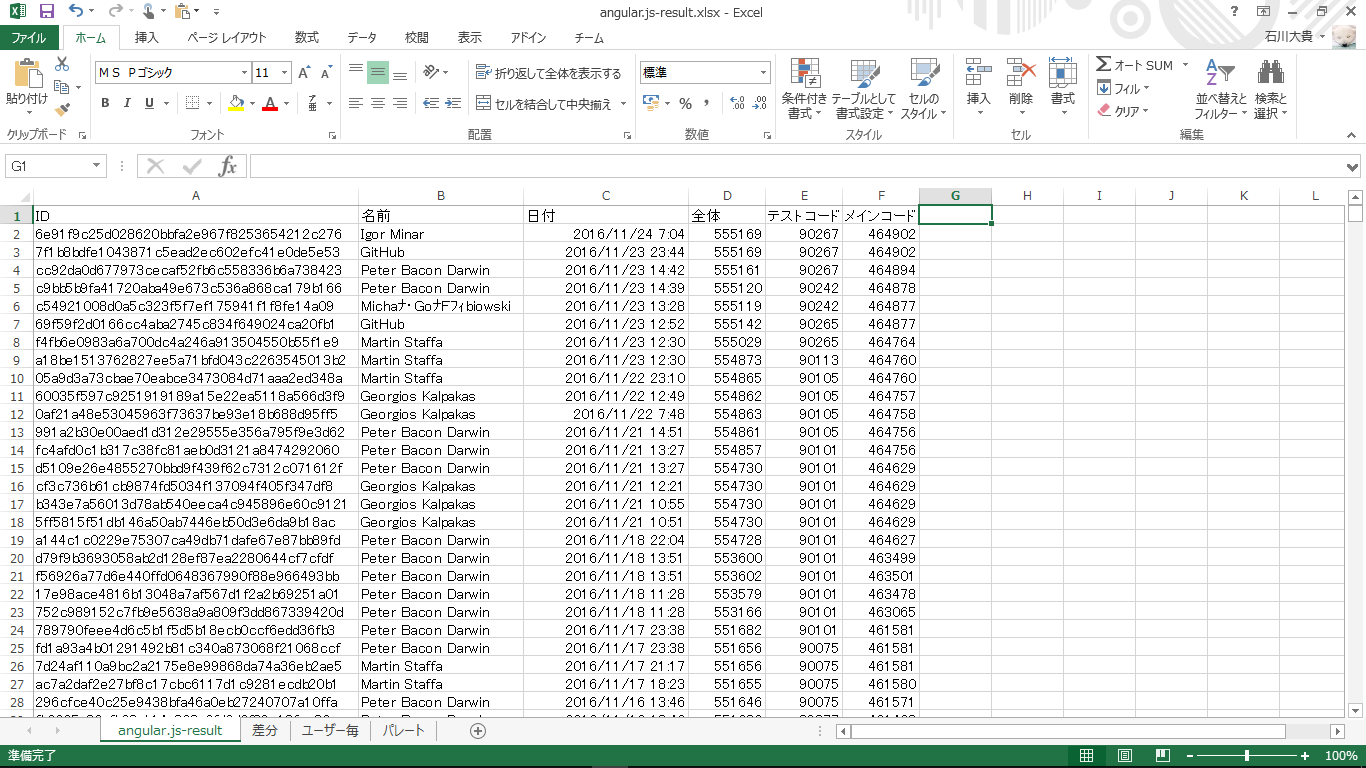
\includegraphics[width=13cm]{process1.png}
\caption{手順1}
\end{figure}

\newpage

新しいコミットから順に並んでいる.コミットごとの追加行数を調べたいので,後のコミットから前のコミットを引いて差分を出せばよい.そのためにまず,古いコミットから順番に並べる.

%図の挿入
\begin{figure}[h]
\centering
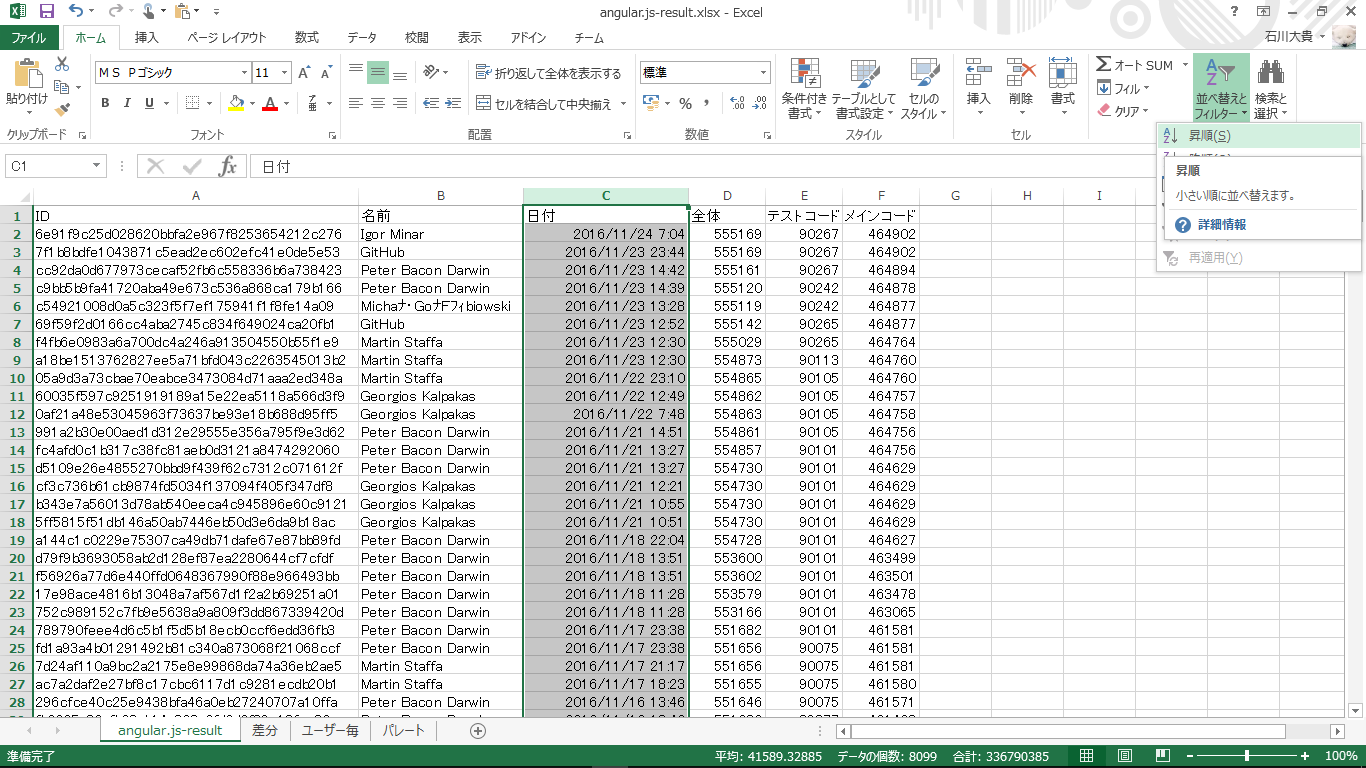
\includegraphics[width=13cm]{process2.png}
\caption{手順2}
\end{figure}

%図の挿入
\begin{figure}[h]
\centering
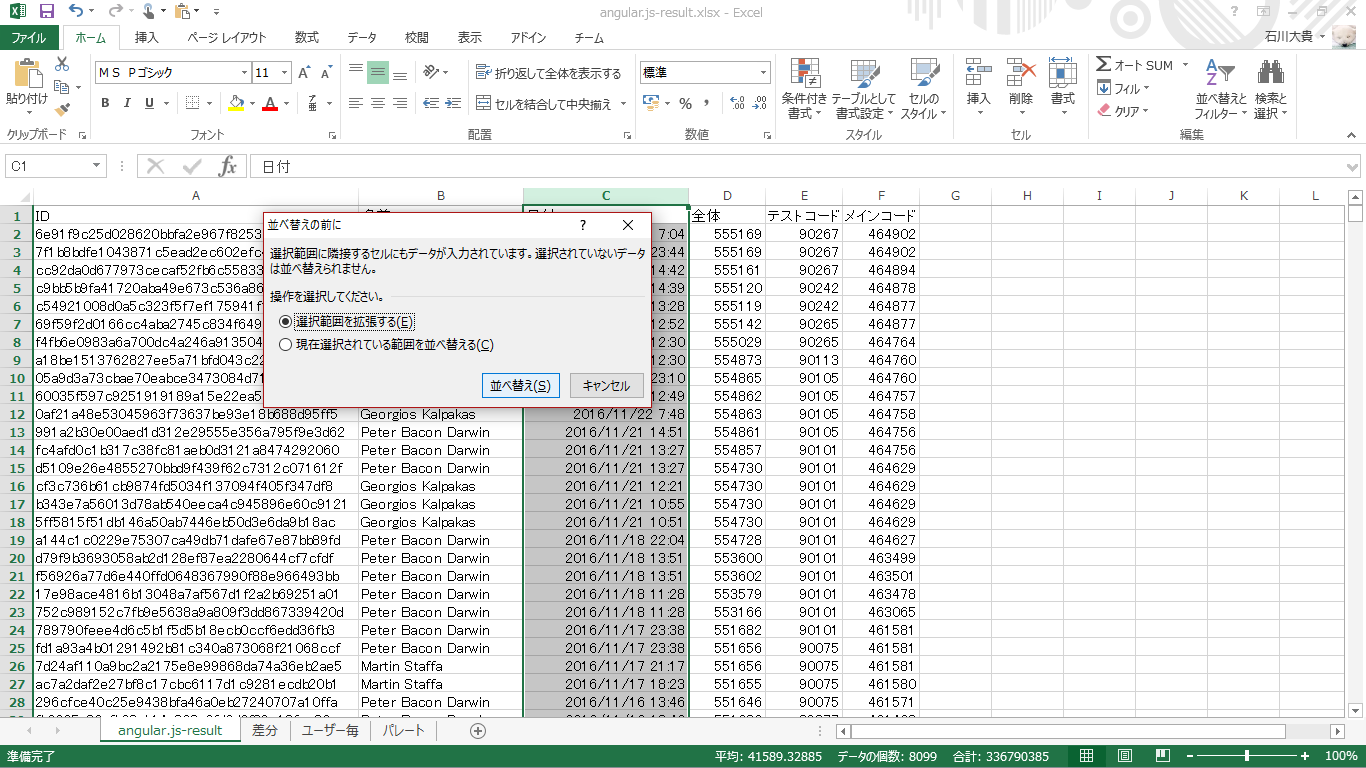
\includegraphics[width=13cm]{process3.png}
\caption{手順3}
\end{figure}

%図の挿入
\begin{figure}[h]
\centering
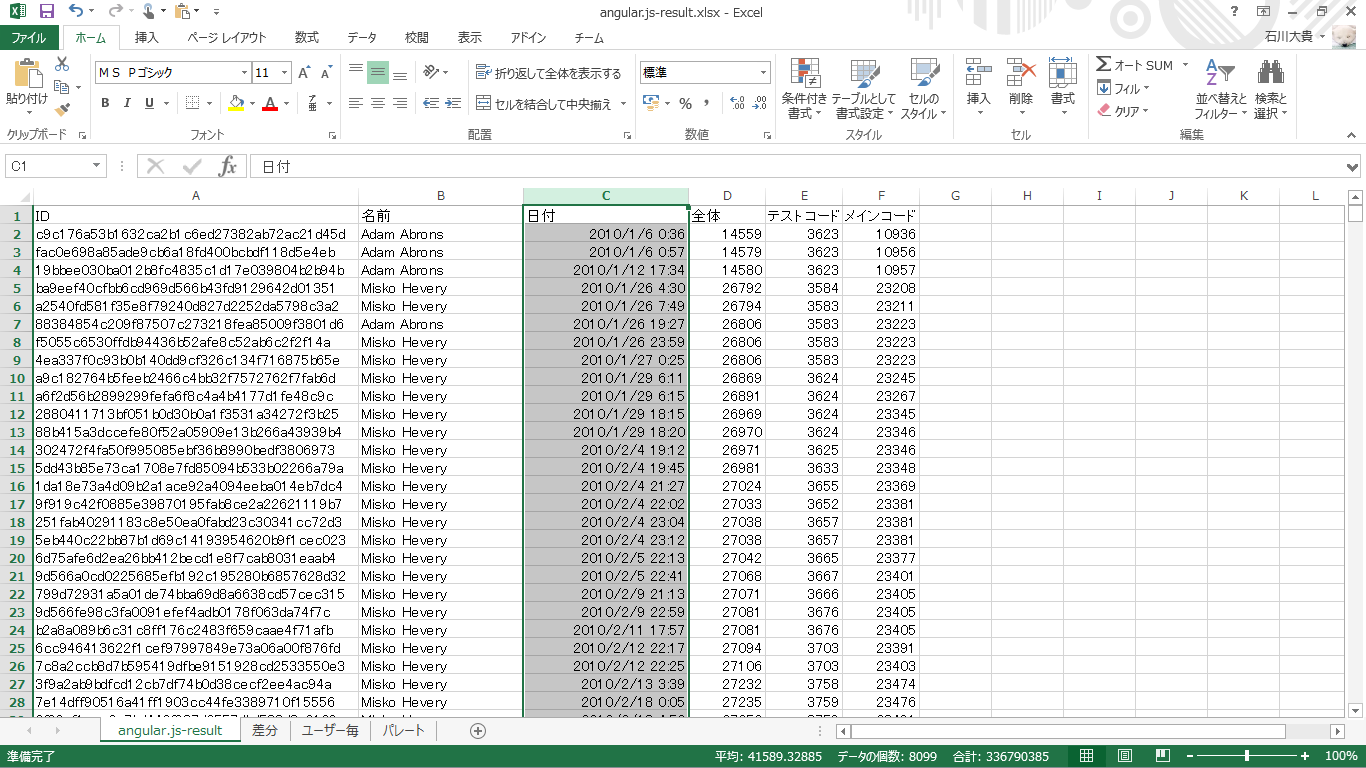
\includegraphics[width=13cm]{process4.png}
\caption{手順4}
\end{figure}

\newpage

テストコードとメインコードの1行目はそのまま隣のセルにコピーする.コピーしたセルの下に後のコミットから前のコミットを引いた結果を出力する.

%図の挿入
\begin{figure}[h]
\centering
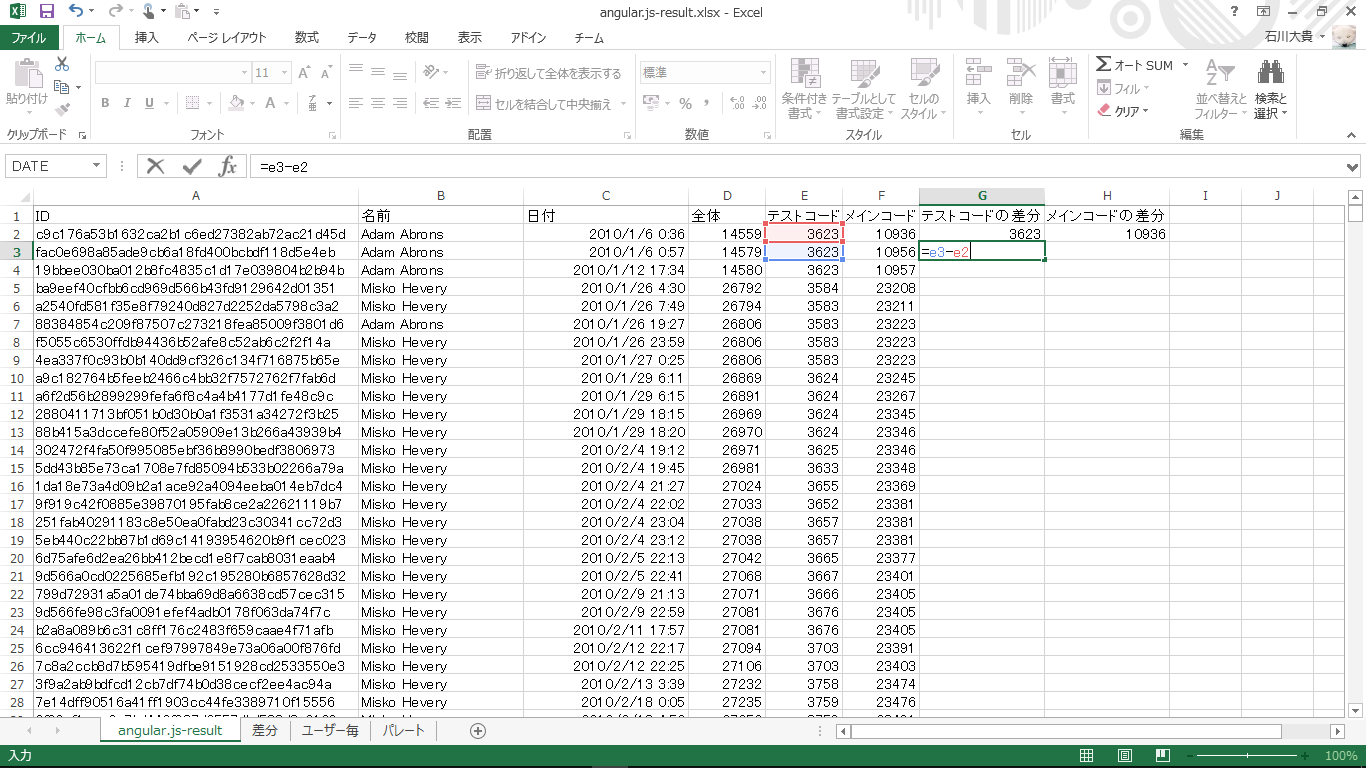
\includegraphics[width=13cm]{process5.png}
\caption{手順5}
\end{figure}

\newpage

手順6の画像のように,赤矢印の方向に引っ張る.青丸で囲んだセルの右下をダブルクリックすることで,数式を書くのは一度で済む.

%図の挿入
\begin{figure}[h]
\centering
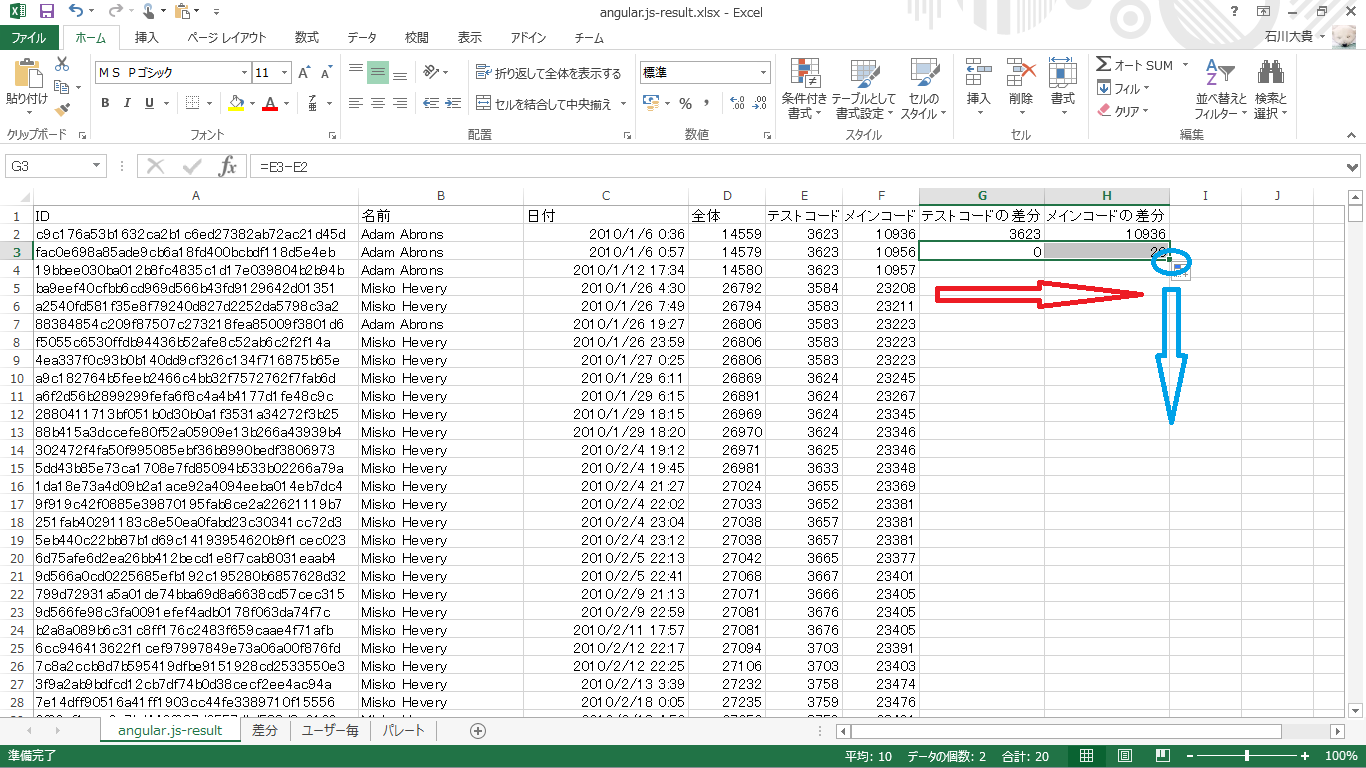
\includegraphics[width=13cm]{process6.png}
\caption{手順6}
\end{figure}

手順7の画像のように,一番下まで全てのコミットの差分が出せればよい.

%図の挿入
\begin{figure}[h]
\centering
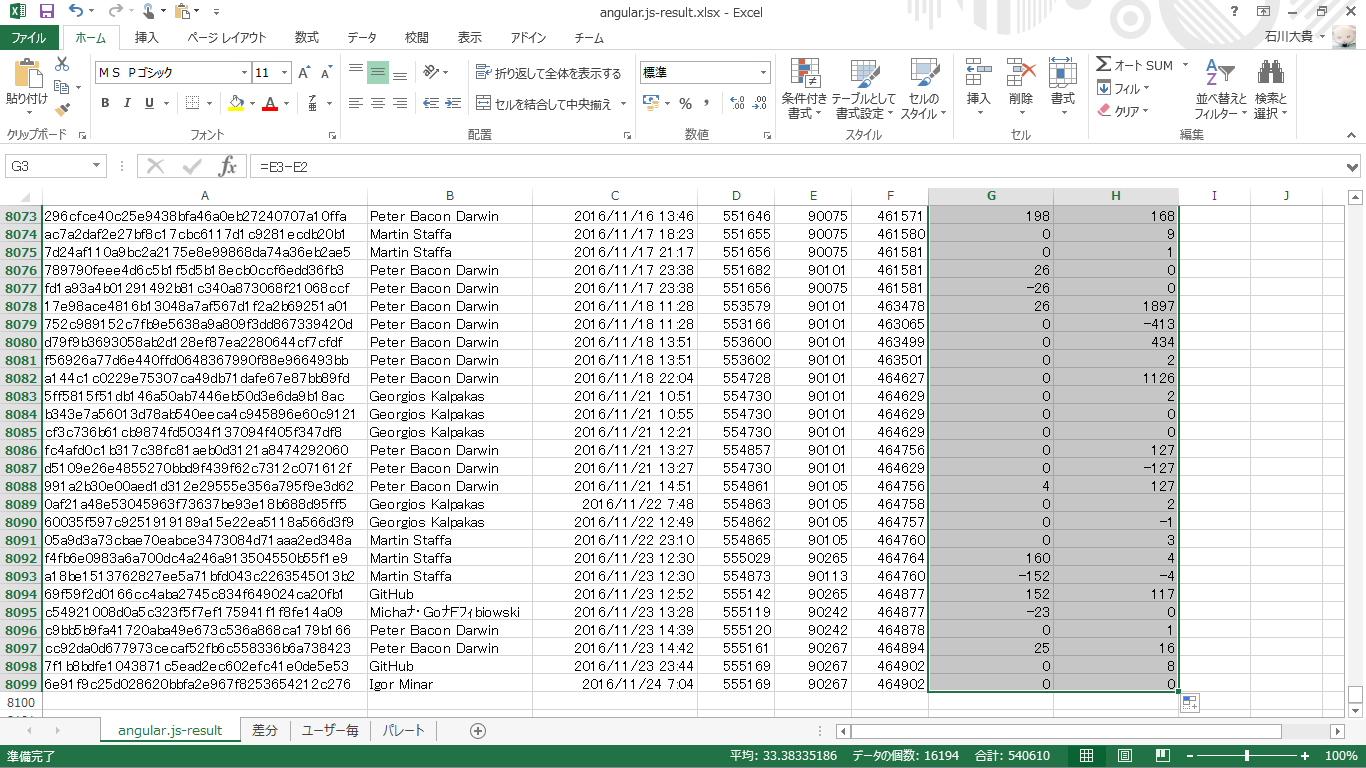
\includegraphics[width=13cm]{process7.png}
\caption{手順7}
\end{figure}

\newpage

作業を行いやすくするため,新しいシートに名前,テストコードとメインコードの差分を移動させる.

%図の挿入
\begin{figure}[h]
\centering
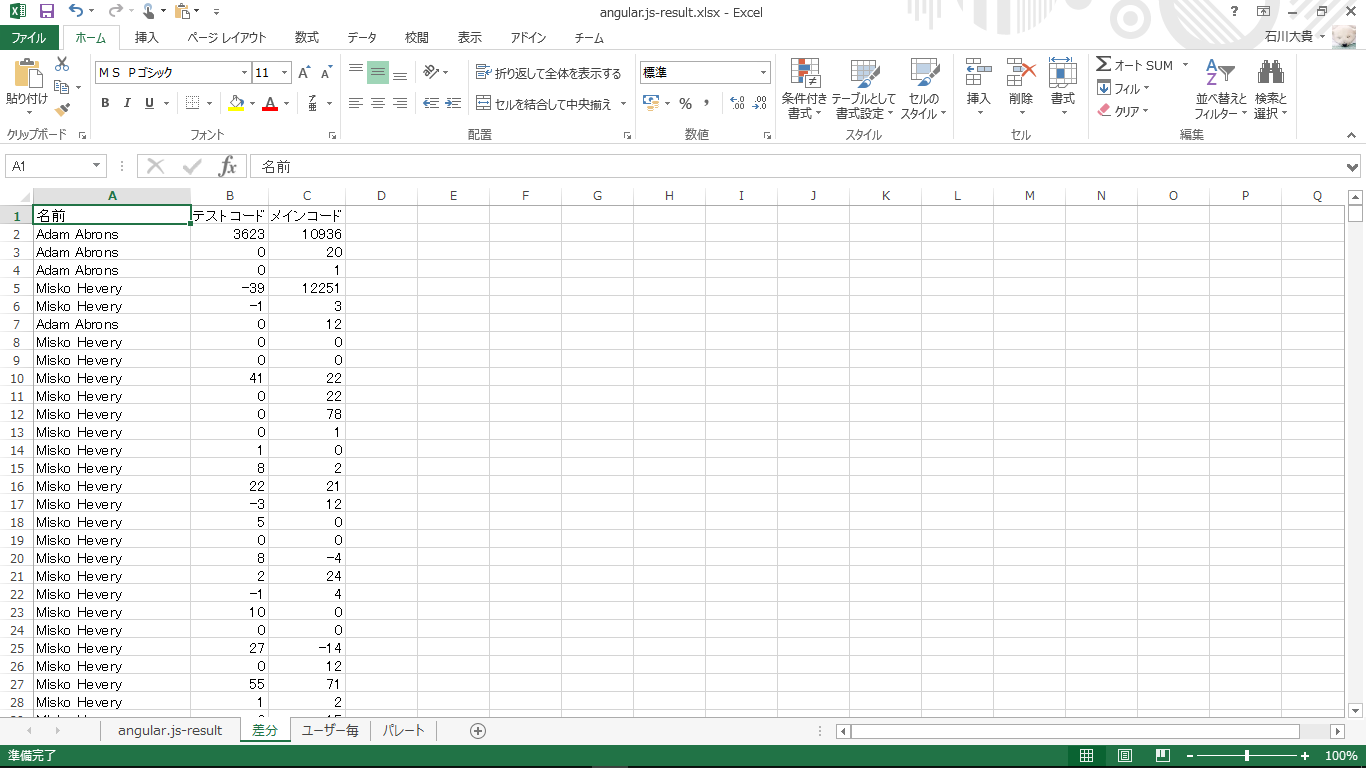
\includegraphics[width=13cm]{process8.png}
\caption{手順8}
\end{figure}

1列目の見出しにフィルターを付ける.

%図の挿入
\begin{figure}[h]
\centering
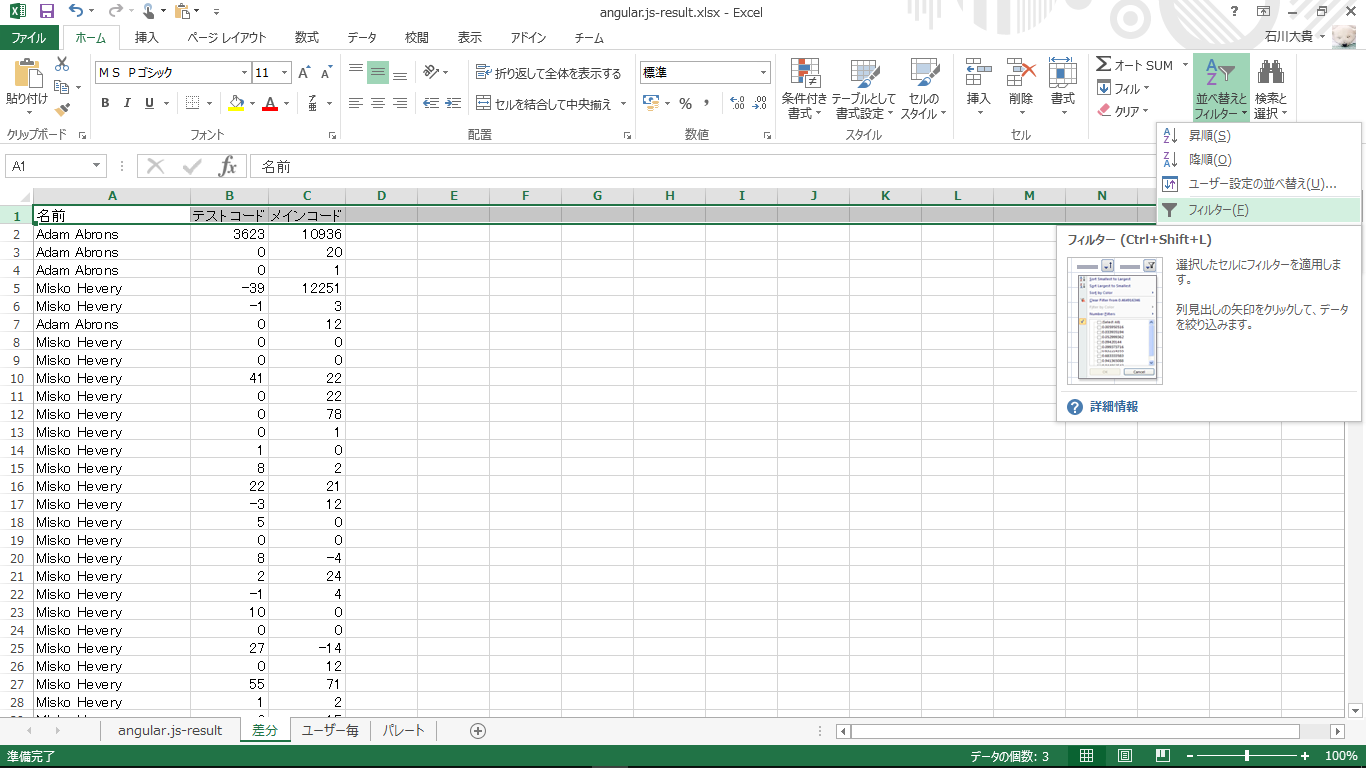
\includegraphics[width=13cm]{process9.png}
\caption{手順9}
\end{figure}

\newpage

1つの名前ごとにフィルターをかける.

%図の挿入
\begin{figure}[h]
\centering
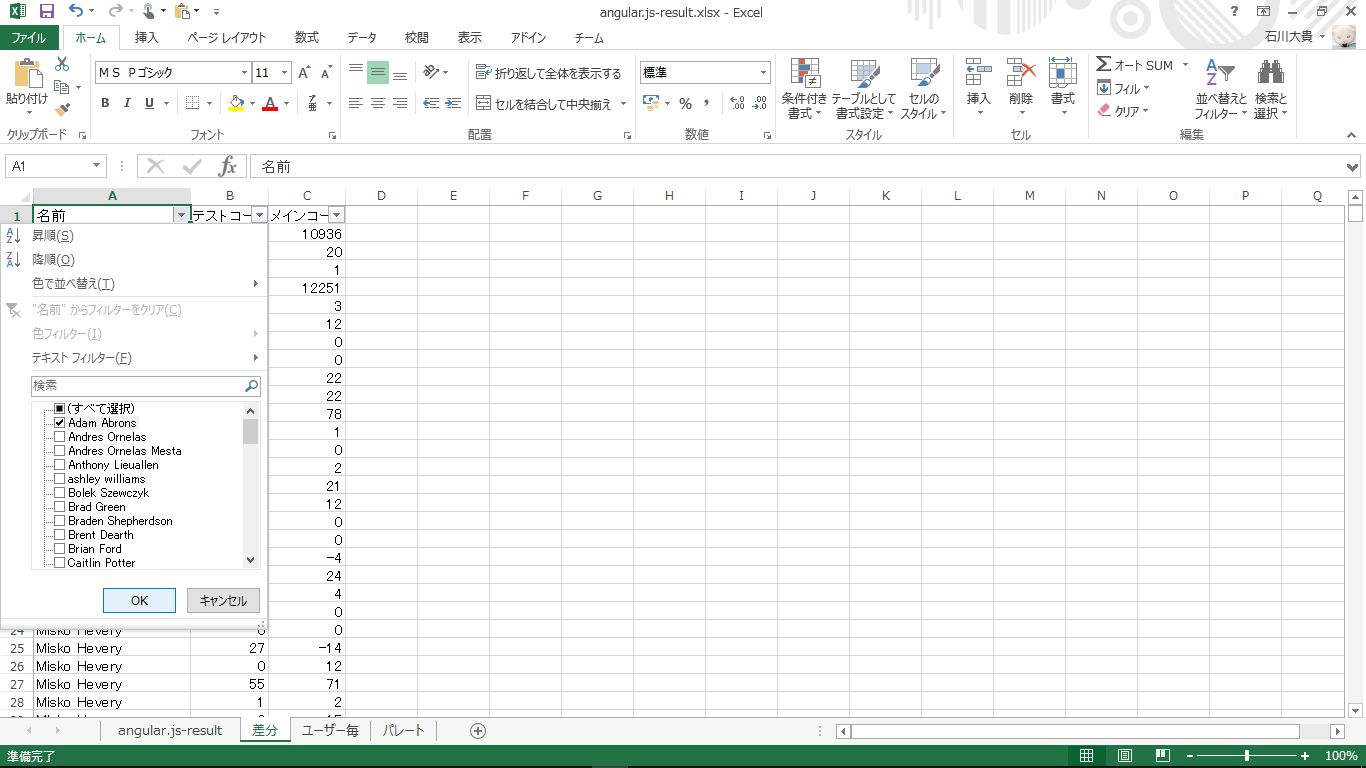
\includegraphics[width=13cm]{process10.png}
\caption{手順10}
\end{figure}

%図の挿入
\begin{figure}[h]
\centering
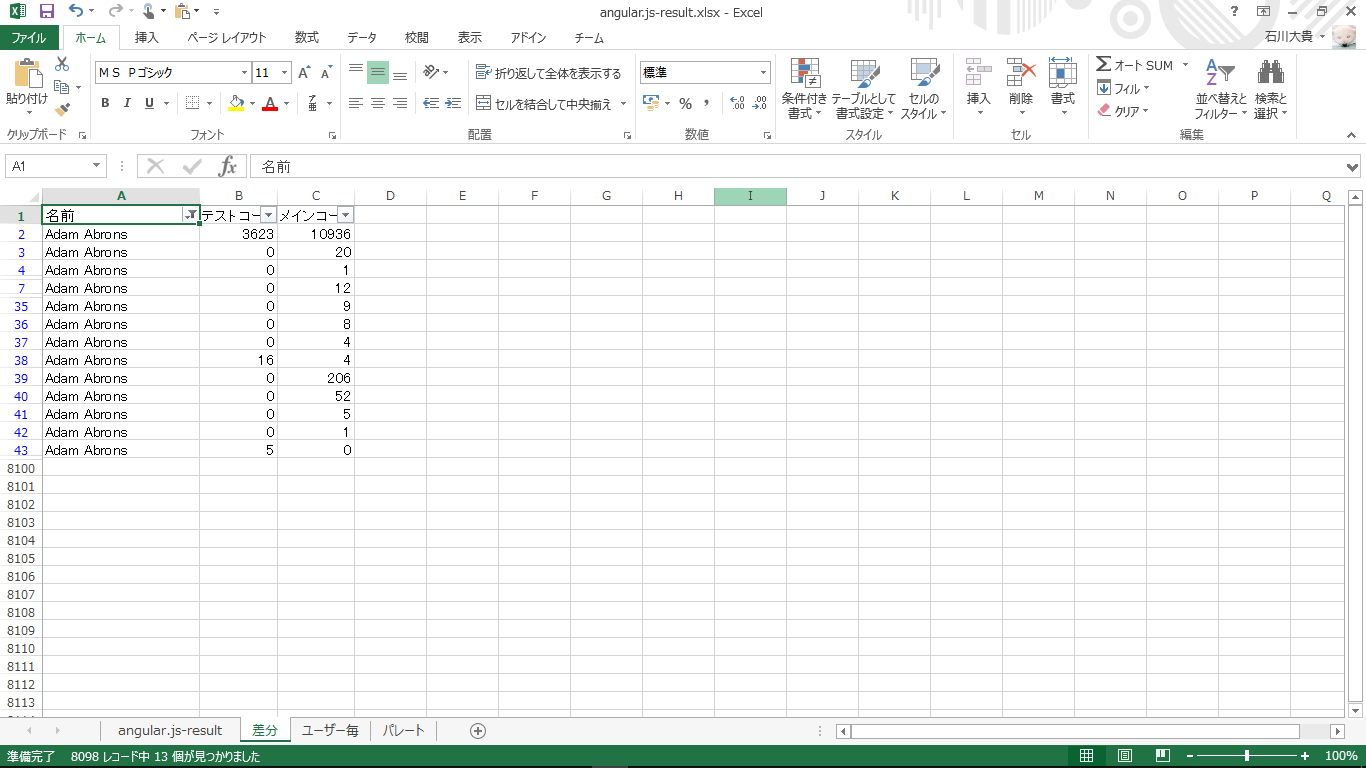
\includegraphics[width=13cm]{process11.png}
\caption{手順11}
\end{figure}

\newpage

テストコードとメインコードの下の空のセルを選択する.オートSUM機能を使いそれぞれの合計を出力する.

%図の挿入
\begin{figure}[h]
\centering
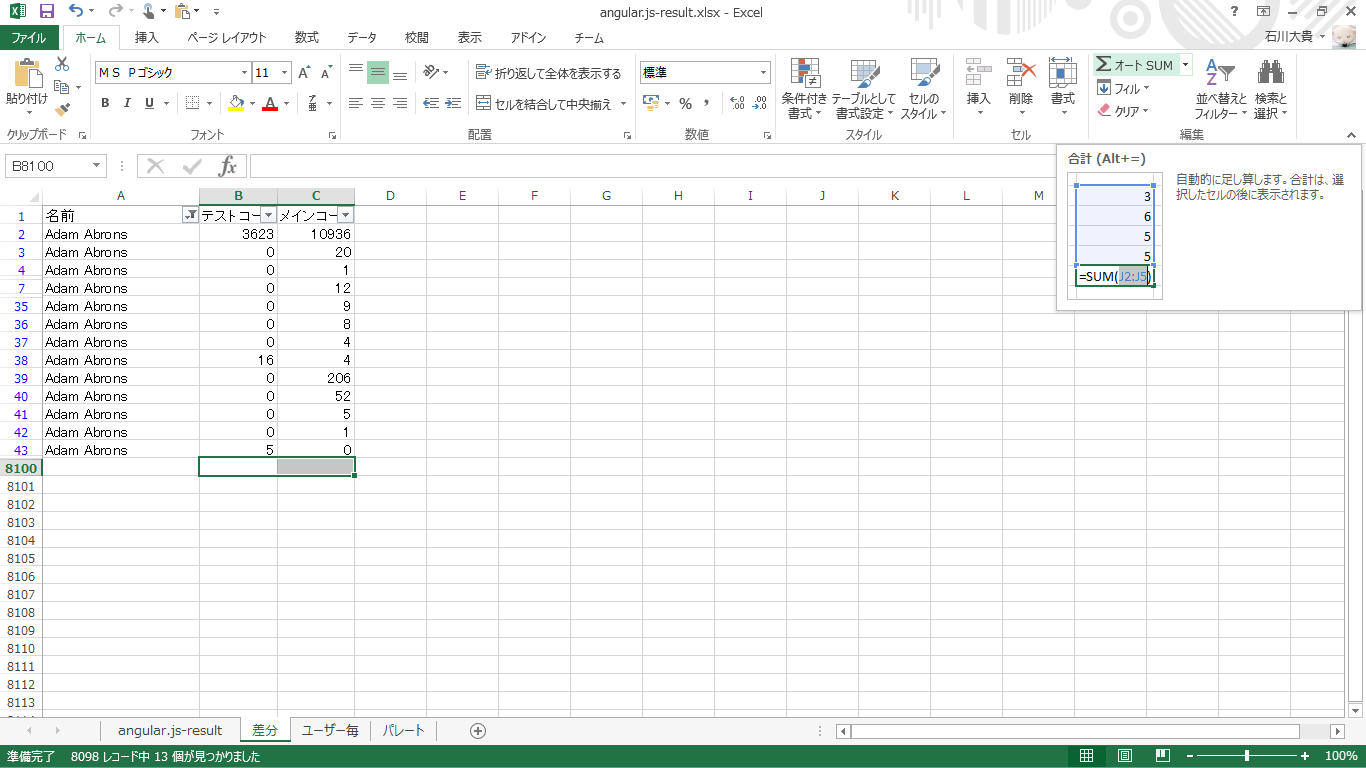
\includegraphics[width=13cm]{process12.png}
\caption{手順12}
\end{figure}

%図の挿入
\begin{figure}[h]
\centering
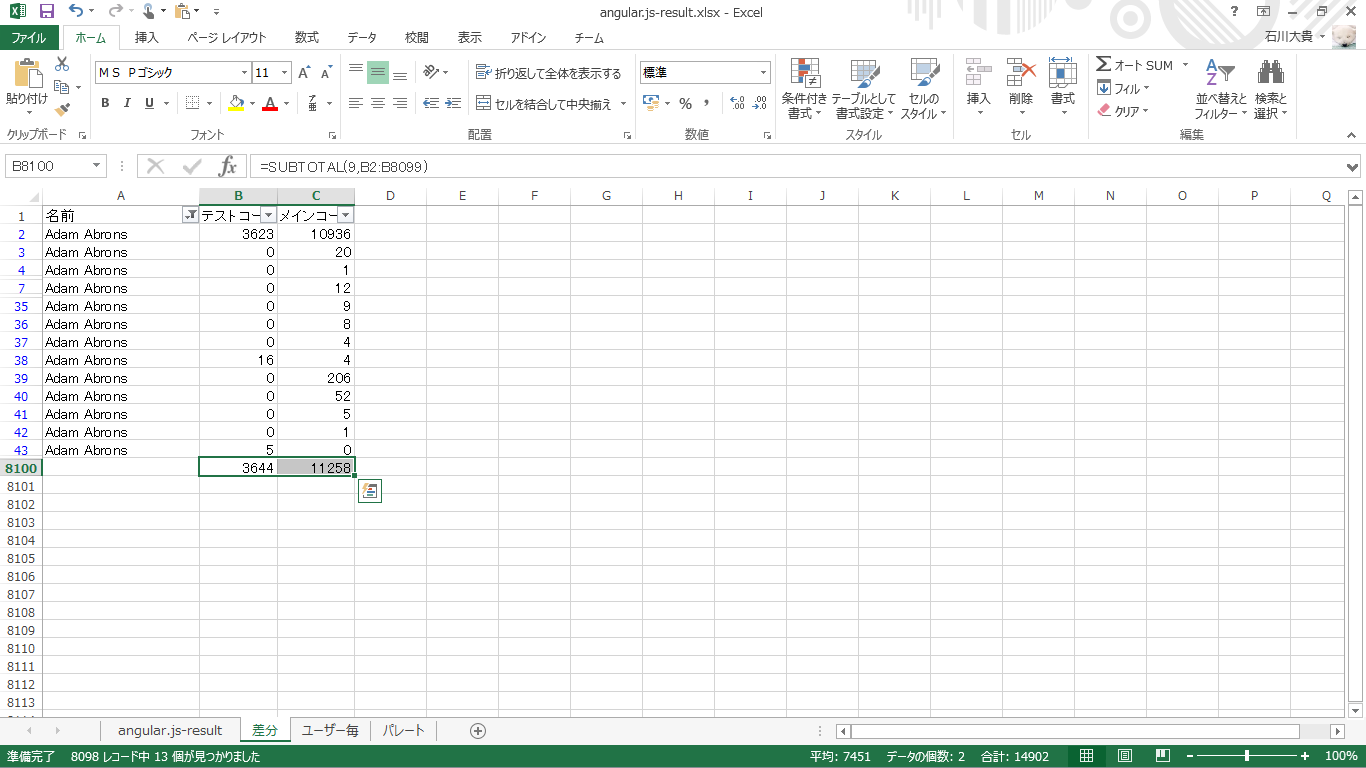
\includegraphics[width=13cm]{process13.png}
\caption{手順13}
\end{figure}

\newpage

新しいシートに名前と出力した合計を記録する.
これを全ての名前を記録するまで行う.

%図の挿入
\begin{figure}[h]
\centering
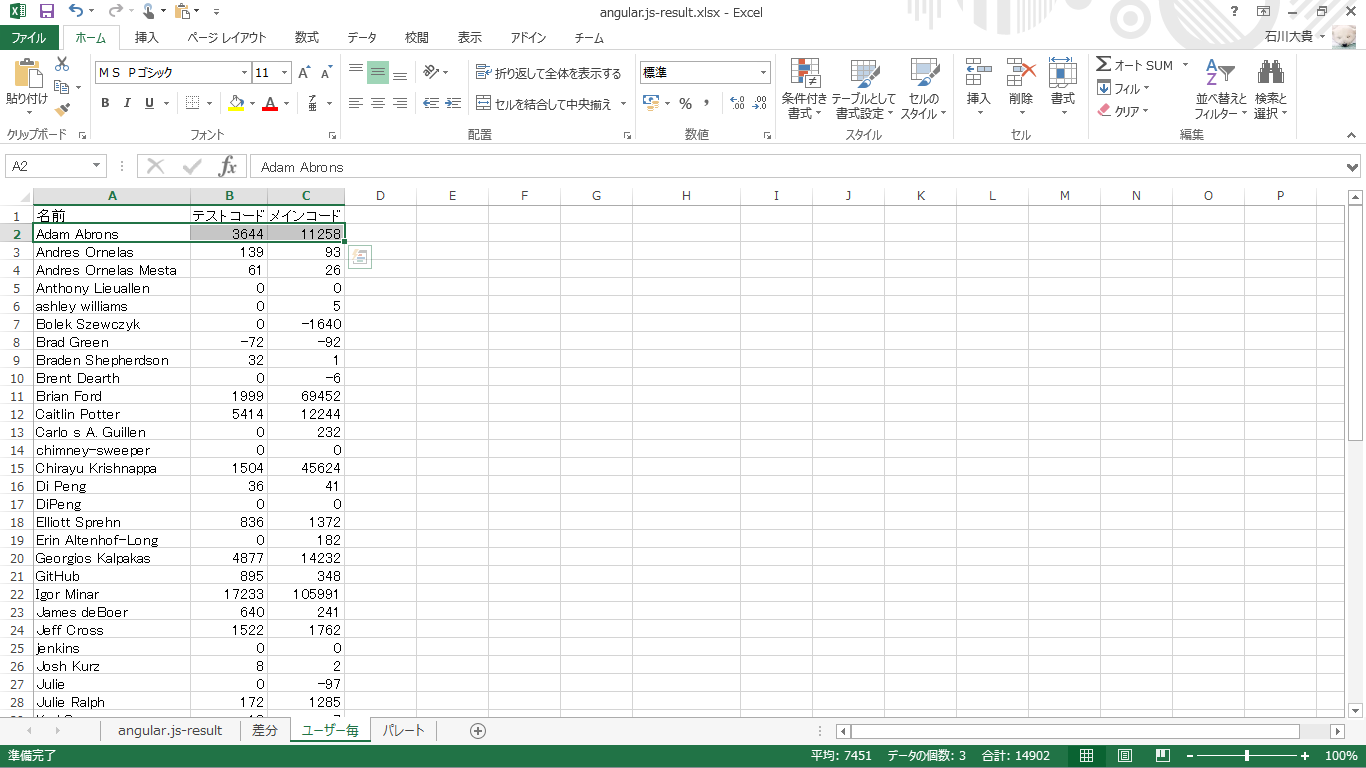
\includegraphics[width=13cm]{process14.png}
\caption{手順14}
\end{figure}

全て記録できたら,テストコードの列を選択し,降順で並べ替える.

%図の挿入
\begin{figure}[h]
\centering
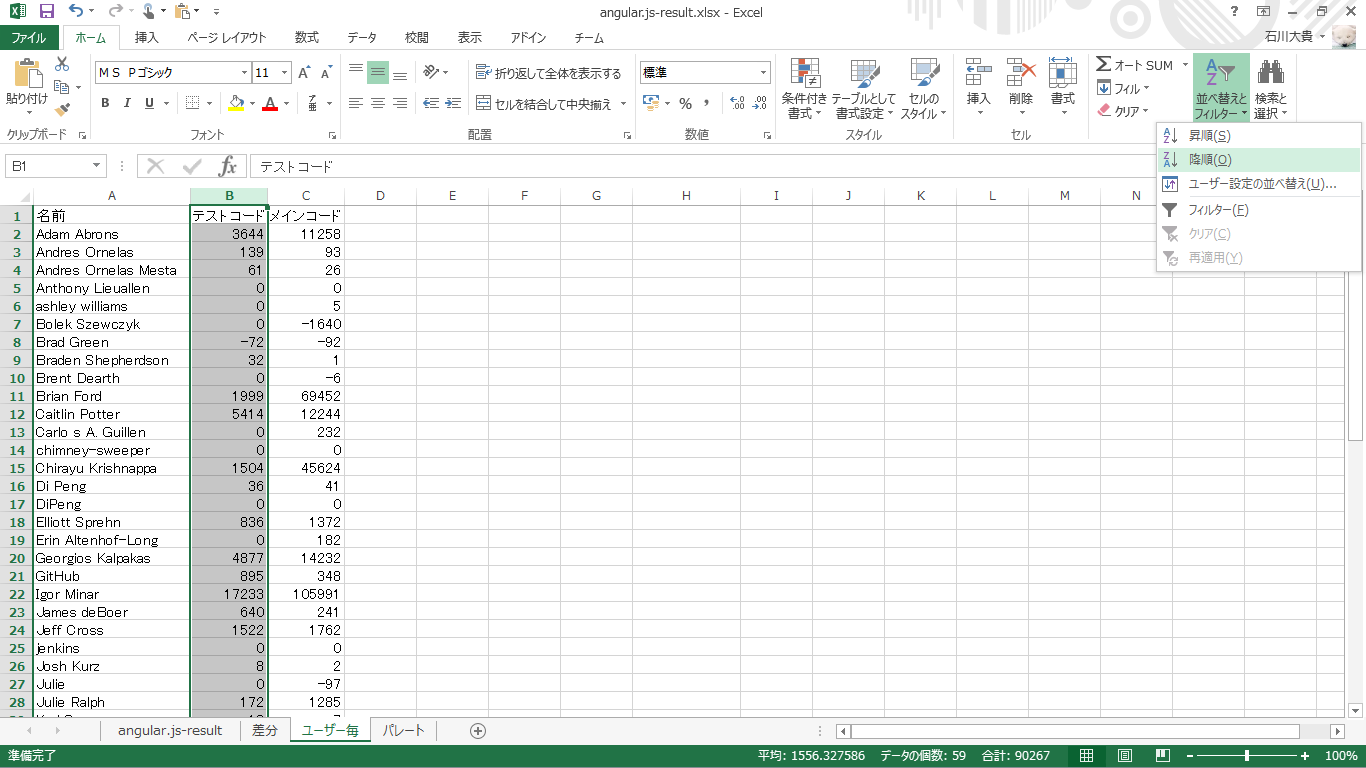
\includegraphics[width=13cm]{process15.png}
\caption{手順15}
\end{figure}

\newpage

テストコードの数字が1以上である範囲のセルを選択し,データの個数と合計を新しいシートに記録する.データの個数は参加者の人数となり,合計は追加されたコード行数の合計となる.

%図の挿入
\begin{figure}[h]
\centering
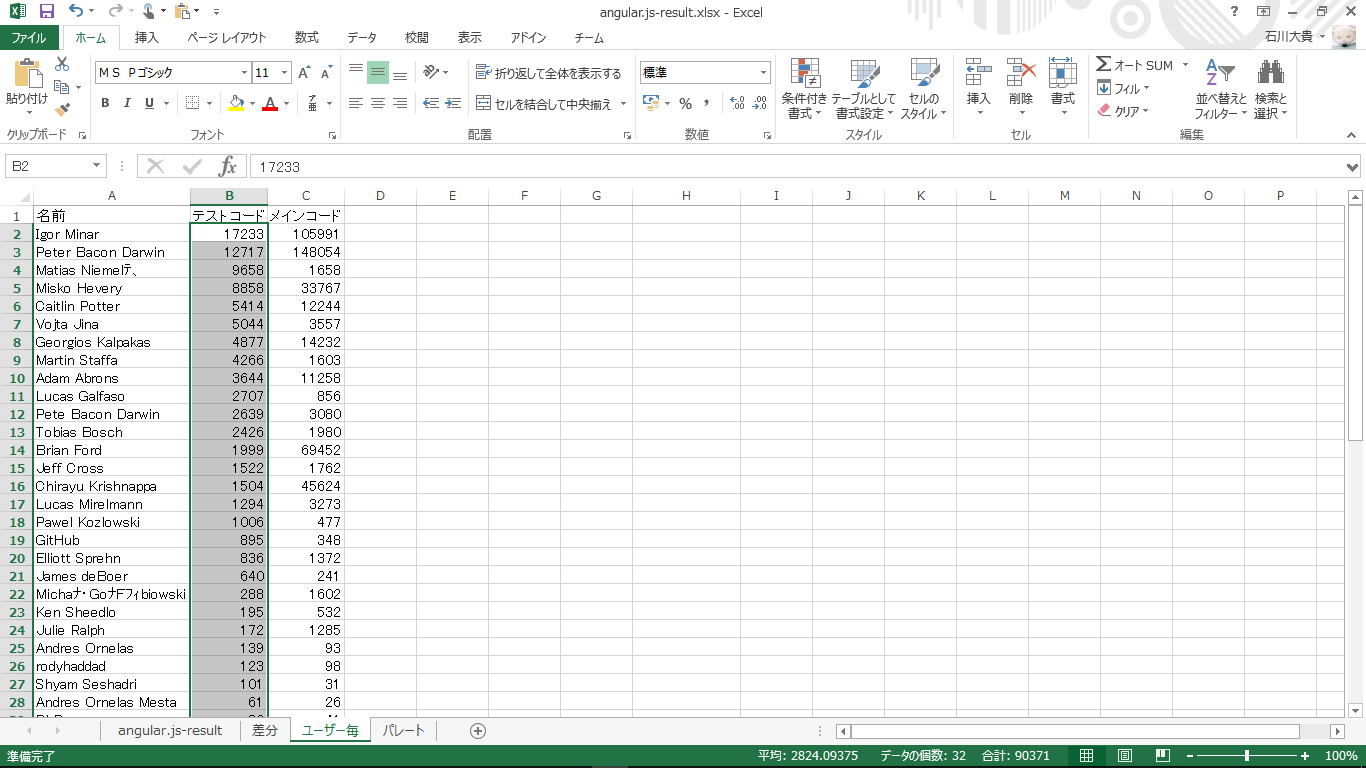
\includegraphics[width=13cm]{process16.png}
\caption{手順16}
\end{figure}

%図の挿入
\begin{figure}[h]
\centering
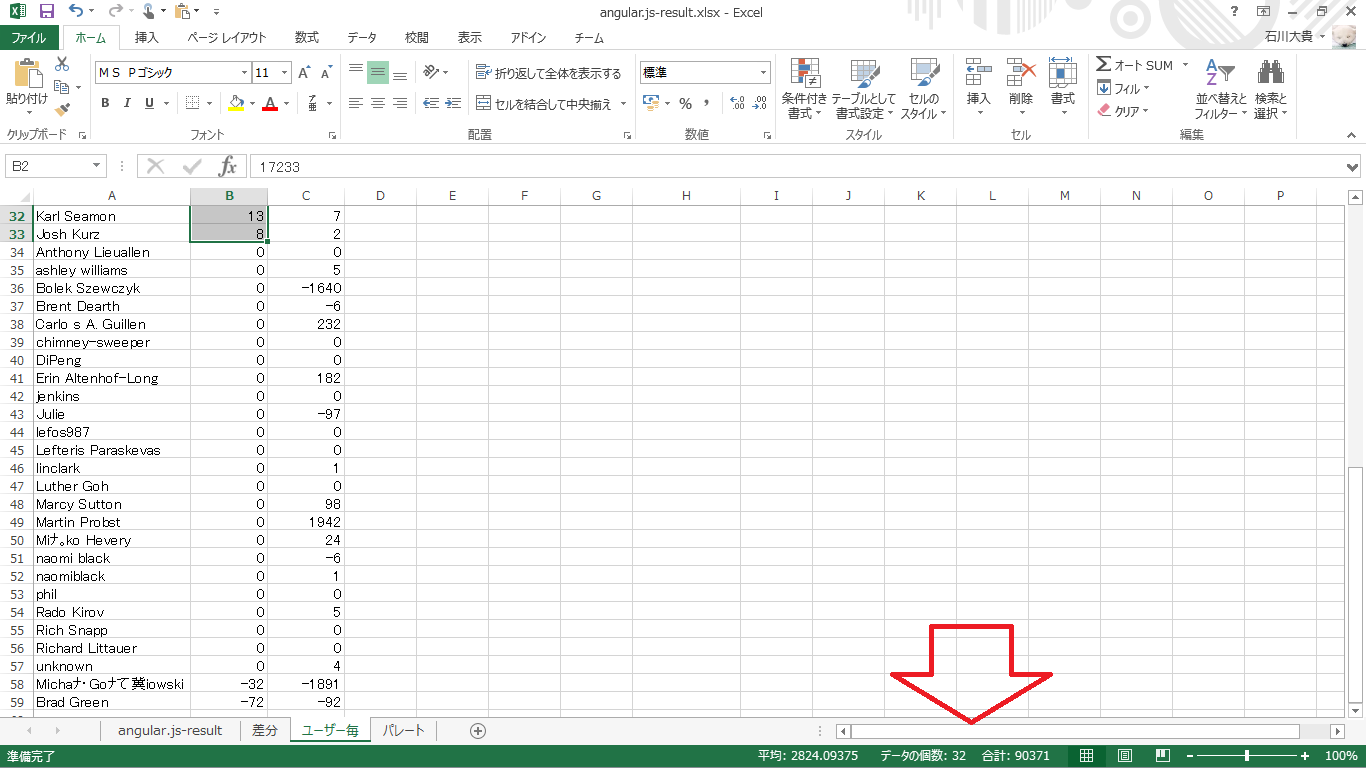
\includegraphics[width=13cm]{process17.png}
\caption{手順17}
\end{figure}

\newpage

メインコードでも同様にして,データの個数と合計を記録する.

%図の挿入
\begin{figure}[h]
\centering
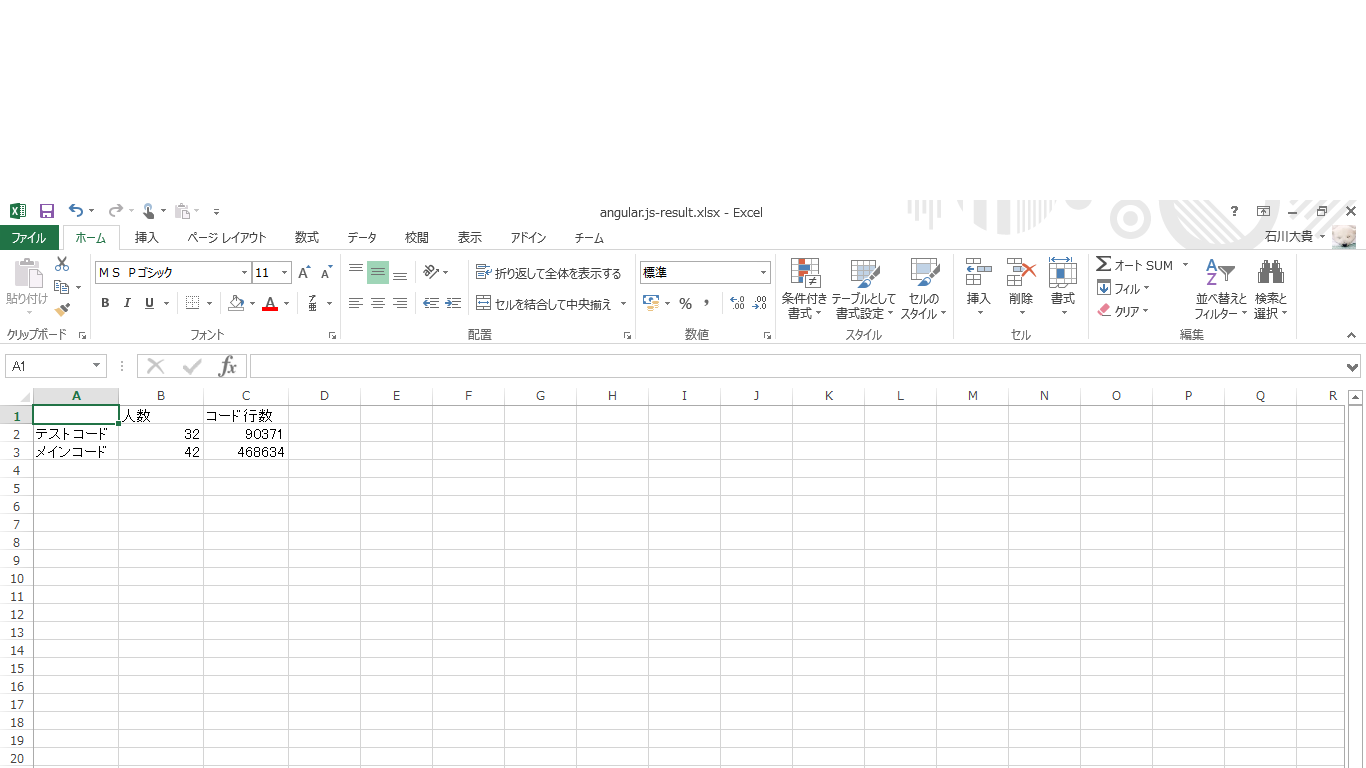
\includegraphics[width=13cm]{process18.png}
\caption{手順18}
\end{figure}

次に,メインコードとテストコードでそれぞれパレートの法則が成り立つのか検証してみる.
80\%以上のコード行数を書いているのが20\%以下のユーザであるときパレートの法則が成り立つとする.

まず,80\%のコード行数を計算する.

%図の挿入
\begin{figure}[h]
\centering
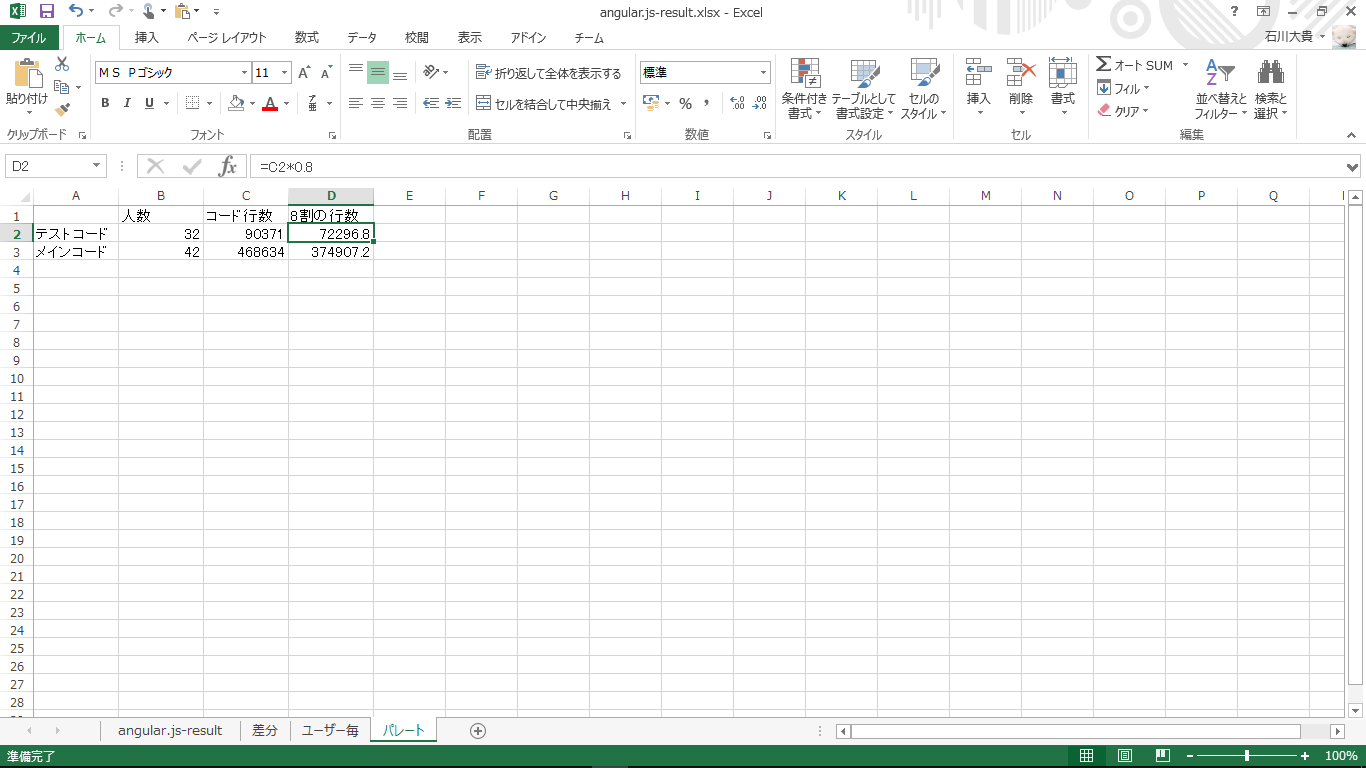
\includegraphics[width=13cm]{process19.png}
\caption{手順19}
\end{figure}

\newpage

前のシートに戻り,複数のセル選択時に表示される合計の数値を確認して,80\%のコード行数を超えるところまでセルを選択する.選択した範囲のデータの個数を記録し,これを上位の貢献者の人数とする.また,この時選択した範囲にいた名前のユーザを上位の貢献者たちとし記録しておく.

%図の挿入
\begin{figure}[h]
\centering
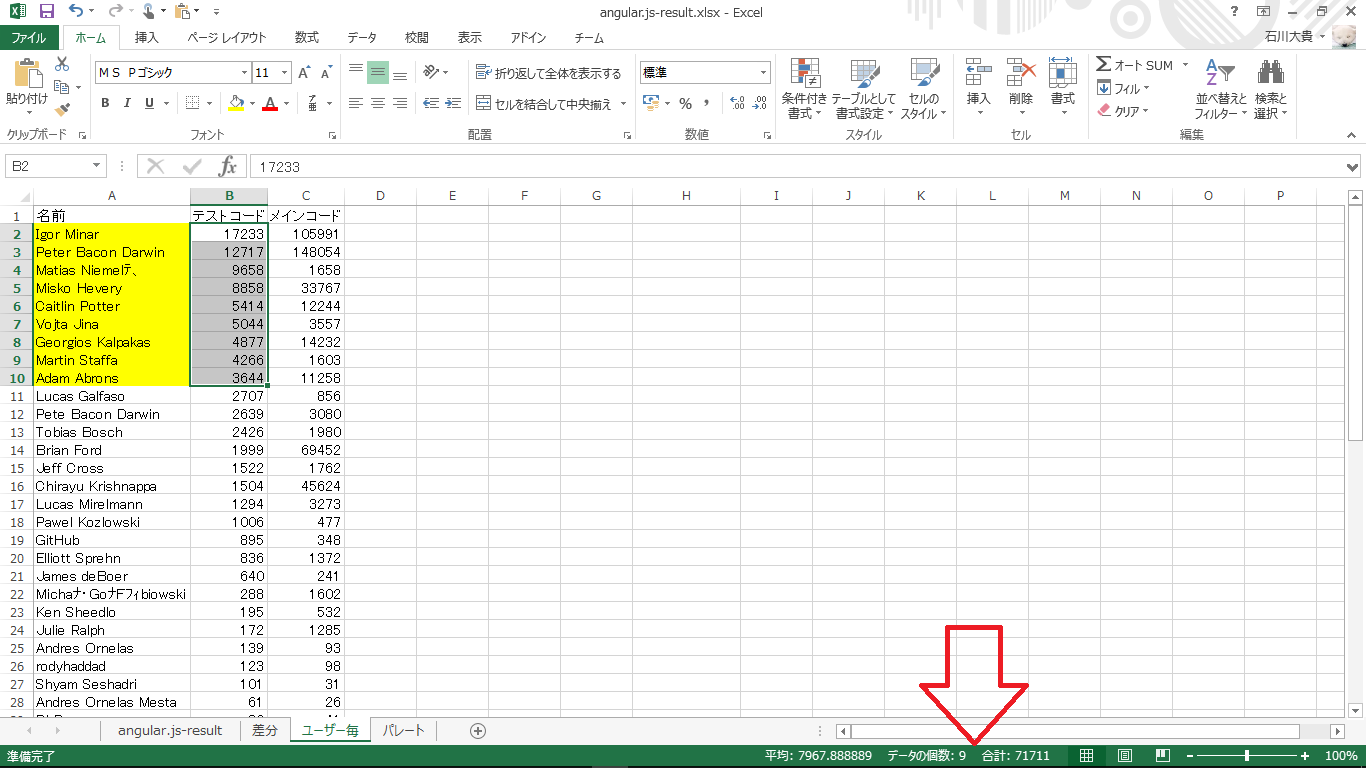
\includegraphics[width=13cm]{process20.png}
\caption{手順20}
\end{figure}

%図の挿入
\begin{figure}[h]
\centering
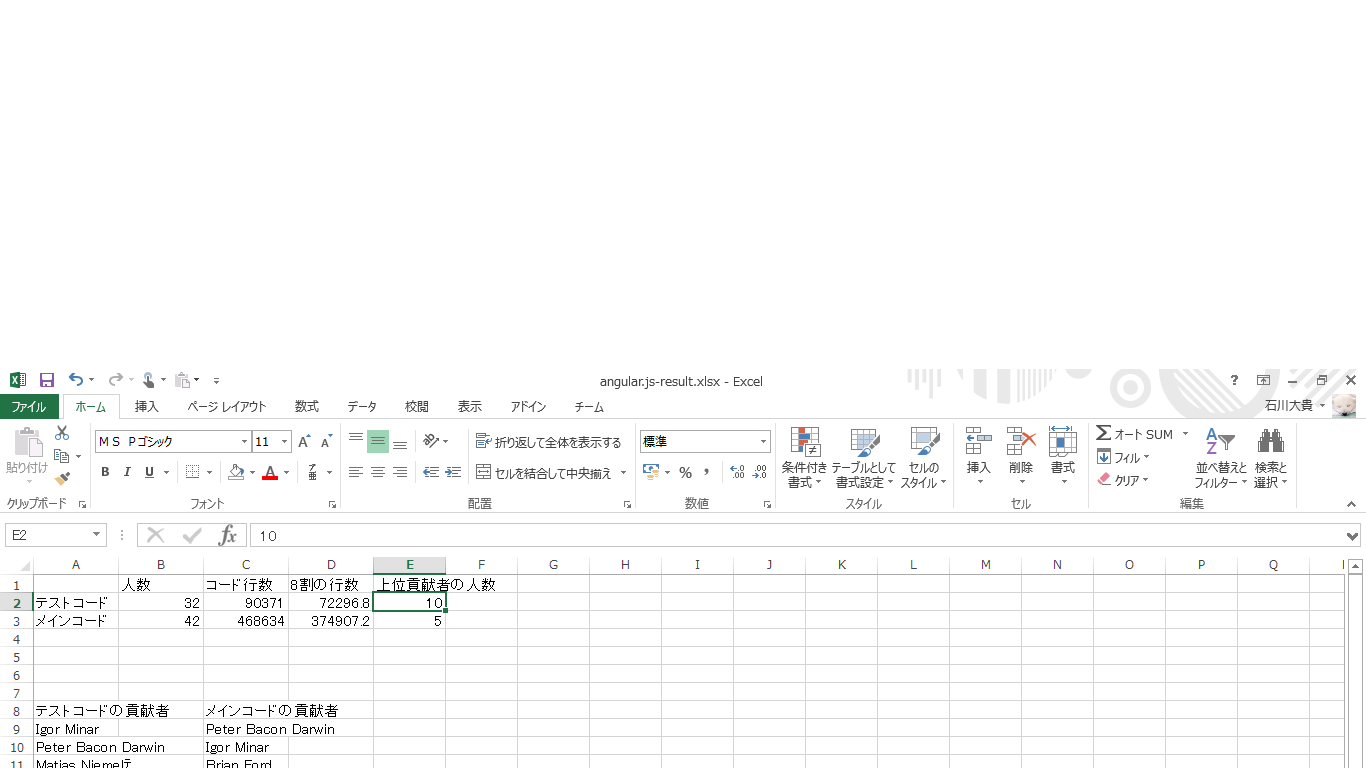
\includegraphics[width=13cm]{process21.png}
\caption{手順21}
\end{figure}

\newpage

上位の貢献者の人数÷参加者の人数を×100を計算して,20\%を下回っていればパレートの法則は成り立つものとする.

%図の挿入
\begin{figure}[h]
\centering
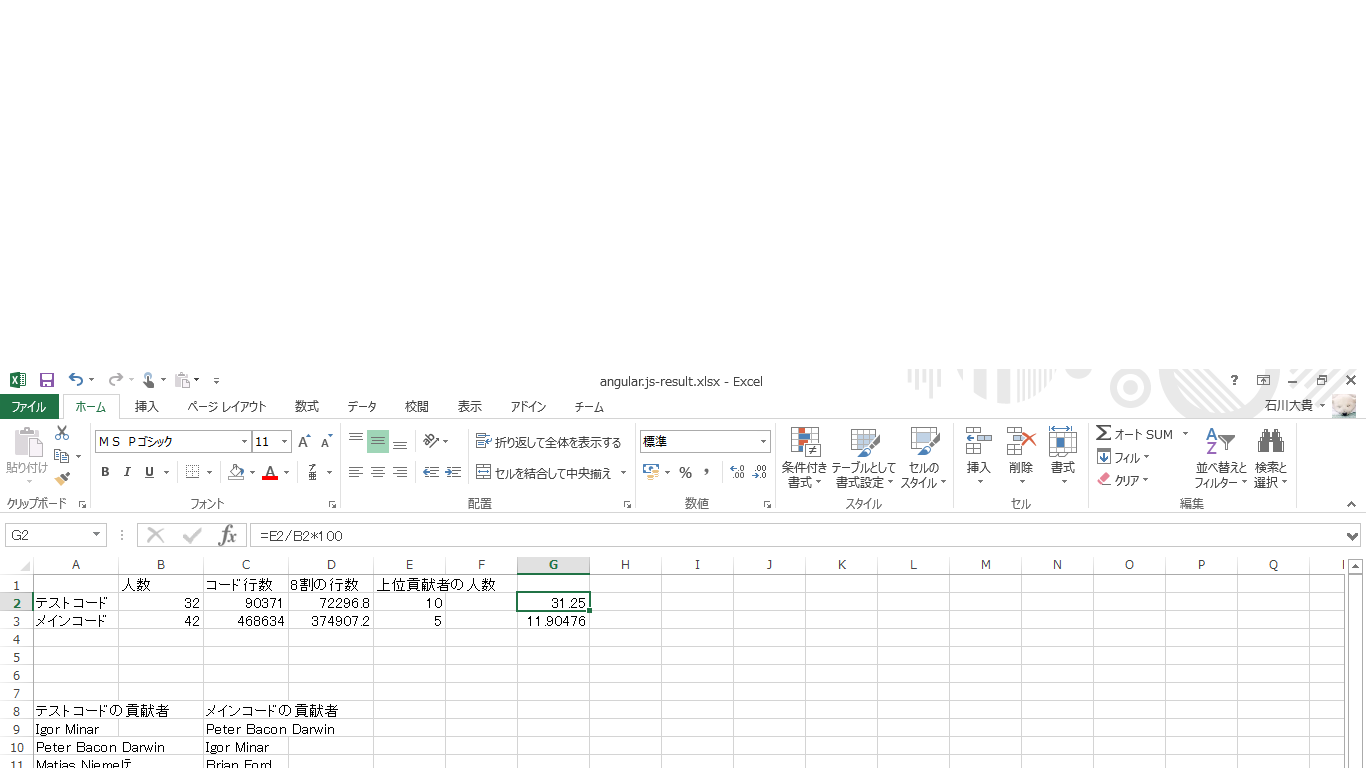
\includegraphics[width=13cm]{process22.png}
\caption{手順22}
\end{figure}

ここまで集計したデータを元に,テストコードとメインコードの上位貢献での同じ人物はいるのか,パレートの法則が成り立つ場合とそうでない場合の違い等を比べてる.



\chapter{結果・考察}

今回22件のプロジェクトを調査した.プロジェクトごとにメンバがそれぞれ追加したコード行数を集計した.集計したデータの一覧を次に記す.

\begin{table}[htb]
\begin{center}
\caption{angular/angular.js - 1}
\begin{tabular}{|l|r|r|} \hline 
名前 & テスト & 本体 \\ \hline \hline
Adam Abrons & 3644 & 11258 \\ \hline
Andres Ornelas & 139 & 93 \\ \hline
Andres Ornelas Mesta & 61 & 26 \\ \hline
Anthony Lieuallen & 0 & 0 \\ \hline
ashley williams & 0 & 5 \\ \hline
Bolek Szewczyk & 0 & -1640 \\ \hline
Brad Green & -72 & -92 \\ \hline
Braden Shepherdson & 32 & 1 \\ \hline
Brent Dearth & 0 & -6 \\ \hline
Brian Ford & 1999 & 69452 \\ \hline
Caitlin Potter & 5414 & 12244 \\ \hline
Carlo s A. Guillen & 0 & 232 \\ \hline
chimney-sweeper & 0 & 0 \\ \hline
Chirayu Krishnappa & 1504 & 45624 \\ \hline
Di Peng & 36 & 41 \\ \hline
DiPeng & 0 & 0 \\ \hline
Elliott Sprehn & 836 & 1372 \\ \hline
Erin Altenhof-Long & 0 & 182 \\ \hline
Georgios Kalpakas & 4877 & 14232 \\ \hline
GitHub & 895 & 348 \\ \hline
Igor Minar & 17233 & 105991 \\ \hline
James deBoer & 640 & 241 \\ \hline
Jeff Cross & 1522 & 1762 \\ \hline
jenkins & 0 & 0 \\ \hline
Josh Kurz & 8 & 2 \\ \hline
Julie & 0 & -97 \\ \hline
Julie Ralph & 172 & 1285 \\ \hline
Karl Seamon & 13 & 7 \\ \hline
Ken Sheedlo & 195 & 532 \\ \hline
lefos987 & 0 & 0 \\ \hline
\end{tabular}
\end{center}
\end{table}

\begin{table}[htb]
\begin{center}
\caption{angular/angular.js - 2}
\begin{tabular}{|l|r|r|} \hline 
名前 & テスト & 本体 \\ \hline \hline
Lefteris Paraskevas & 0 & 0 \\ \hline
linclark & 0 & 1 \\ \hline
Lucas Galfaso & 2707 & 856 \\ \hline
Lucas Mirelmann & 1294 & 3273 \\ \hline
Luther Goh & 0 & 0 \\ \hline
Marcy Sutton & 0 & 98 \\ \hline
Martin Probst & 0 & 1942 \\ \hline
Martin Staffa & 4266 & 1603 \\ \hline
Matias Niemelテ、 & 9658 & 1658 \\ \hline
Michaナ・GoナFフィbiowski & 288 & 1602 \\ \hline
Michaナ・Goナて冀iowski & -32 & -1891 \\ \hline
Misko Hevery & 8858 & 33767 \\ \hline
Miナ。ko Hevery & 0 & 24 \\ \hline
naomi black & 0 & -6 \\ \hline
naomiblack & 0 & 1 \\ \hline
Pawel Kozlowski & 1006 & 477 \\ \hline
Pete Bacon Darwin & 2639 & 3080 \\ \hline
Peter Bacon Darwin & 12717 & 148054 \\ \hline
phil & 0 & 0 \\ \hline
Rado Kirov & 0 & 5 \\ \hline
Rich Snapp & 0 & 0 \\ \hline
Richard Littauer & 0 & 0 \\ \hline
rodyhaddad & 123 & 98 \\ \hline
Shahar Talmi & 24 & 1593 \\ \hline
Shyam Seshadri & 101 & 31 \\ \hline
Tobias Bosch & 2426 & 1980 \\ \hline
unknown & 0 & 4 \\ \hline
Vojta Jina & 5044 & 3557 \\ \hline
\end{tabular}
\end{center}
\end{table}

\begin{table}[htb]
\begin{center}
\caption{caolan/async}
\begin{tabular}{|l|r|r|} \hline 
名前 & テスト & 本体 \\ \hline \hline
Alex Early & -702 & 3396\\ \hline
Alex Ianus & 0 & 32\\ \hline
Alexander Early & -2397 & 23834\\ \hline
Allan Carroll & 4 & 0\\ \hline
Beau Gunderson & 124 & 117\\ \hline
Caolan McMahon & 3043 & 4904\\ \hline
GitHub & 0 & 102\\ \hline
Graeme Yeates & -159 & 3215\\ \hline
Hubert Argasinski & 0 & 334\\ \hline
MaZderMind & 24 & 14\\ \hline
megawac & 63 & -1\\ \hline
Peter & 0 & 3\\ \hline
\end{tabular}
\end{center}
\end{table}

\begin{table}[htb]
\begin{center}
\caption{jashkenas/backbone - 1}
\begin{tabular}{|l|r|r|} \hline 
名前 & テスト & 本体 \\ \hline \hline
Adam Krebs & 3144 & 181\\ \hline
Aitor Guevara Escalante & 29 & 22\\ \hline
Andrei Bocan & 0 & 17\\ \hline
Andrew Schaaf & 0 & 5\\ \hline
Brad Dunbar & 861 & 341\\ \hline
Casey Foster & 210 & 39\\ \hline
Dmitry Baranovskiy & 0 & 73\\ \hline
dxgriffiths & 0 & 23\\ \hline
Elijah Insua & 0 & 12\\ \hline
Fテゥlix & 0 & 0\\ \hline
Fテゥlix Horro Pita & 0 & 0\\ \hline
GitHub & 24140 & 16144\\ \hline
Graeme & 15 & 11\\ \hline
Graeme Yeates & -1 & 6\\ \hline
Harry Wolff & 0 & 0\\ \hline
Jamie Rolfs & 51 & 4\\ \hline
Jason Davies & 0 & -56\\ \hline
Jeremy Ashkenas & 18467 & 15254\\ \hline
Joshua Peek & 97 & 49\\ \hline
Justin Ridgewell & 24 & 65\\ \hline
Kris Jordan & 13 & 3\\ \hline
Maksim Horbachevsky & 17 & 1\\ \hline
Matt & 9 & -1\\ \hline
michalkot & 11 & -4\\ \hline
Nick Fitzgerald & 90 & 13\\ \hline
Niels Sandholt Busch & 0 & -1\\ \hline
Ofer Nave & 0 & 0\\ \hline
Ore Landau & 0 & 2\\ \hline
Paul Uithol & 68 & 68\\ \hline
Raimonds Simanovskis & 10 & 0\\ \hline
\end{tabular}
\end{center}
\end{table}

\begin{table}[htb]
\begin{center}
\caption{jashkenas/backbone - 2}
\begin{tabular}{|l|r|r|} \hline 
Sam Breed & 9 & -1\\ \hline
Sam Stephenson & 22 & 8\\ \hline
Samuel Clay & 0 & 0\\ \hline
Ted Han & 0 & 1\\ \hline
Tim Branyen & 0 & -3\\ \hline
Tim Griesser & 992 & 12\\ \hline
Ville Lautanala & 2 & 1\\ \hline
Will Moffat & 0 & 5\\ \hline
\end{tabular}
\end{center}
\end{table}

\begin{table}[htb]
\begin{center}
\caption{bower/bower}
\begin{tabular}{|l|r|r|} \hline 
名前 & テスト & 本体 \\ \hline \hline
Adam Stankiewicz & 5241 & 7472\\ \hline
addyosmani & 0 & 0\\ \hline
Alireza Bashiri & 72 & 26\\ \hline
Andre Cruz & 267 & 294\\ \hline
Andreフ・Cruz & 3853 & 5186\\ \hline
Andrテゥ Cruz & 1858 & 960\\ \hline
Ben & 0 & 0\\ \hline
Ben Schwarz & 0 & 4\\ \hline
Chris Aniszczyk & 234 & 1868\\ \hline
Dan Heberden & 36 & 16\\ \hline
David DeSandro & 0 & 21\\ \hline
fat & 205 & 224\\ \hline
GitHub & 0 & 0\\ \hline
Jacob Thornton & 197 & 242\\ \hline
Jaime Olmo & 209 & 28\\ \hline
Mat Scales & 0 & 60\\ \hline
Nicolas Gallagher & 1593 & 779\\ \hline
Paul Irish & 31 & 250\\ \hline
Rob Simpson & 61 & 12\\ \hline
Rod Vagg & 0 & 0\\ \hline
Sindre Sorhus & 424 & 161\\ \hline
Vlad Filippov & 0 & 19\\ \hline
\end{tabular}
\end{center}
\end{table}

\begin{table}[htb]
\begin{center}
\caption{adobe/brackets}
\begin{tabular}{|l|r|r|} \hline 
名前 & テスト & 本体 \\ \hline \hline
名前 & テスト & 本体\\ \hline
Adam Lehman & 0 & 22\\ \hline
Arno Gourdol & 218 & 291\\ \hline
Arun Bose & 1364 & 7451\\ \hline
Arzhan Kinzhalin & 638 & 3234\\ \hline
Bernhard Sirlinger & 3628 & 1953\\ \hline
Bryan Chin & 0 & 33\\ \hline
Chema & 83 & 412\\ \hline
Dennis Kehrig & 1510 & 7452\\ \hline
ficristo & 0 & 204\\ \hline
GitHub & 0 & 208\\ \hline
Glenn Ruehle & 23083 & 51311\\ \hline
Ian Wehrman & 329 & 60\\ \hline
Ingo Richter & 4162 & 48910\\ \hline
Jason San Jose & 5897 & 2708\\ \hline
Jochen Hagenstroem & 0 & 522\\ \hline
julianasuh & 383 & 659\\ \hline
jzhang & 949 & 2227\\ \hline
Kevin Dangoor & 31921 & 156722\\ \hline
Marcel Gerber & 232 & 3247\\ \hline
Miguel Castillo & 297 & 2533\\ \hline
Narciso Jaramillo & 9755 & 29025\\ \hline
nethip & 31 & 303\\ \hline
njadbe & 0 & 3756\\ \hline
Pete Nykテ、nen & 268 & -919\\ \hline
Peter Flynn & 383 & 433\\ \hline
Peter Thiess & 12955 & -2590\\ \hline
Prashanth Nethi & -41 & 2445\\ \hline
pthiess & -41 & 422\\ \hline
Randy Edmunds & 272 & 533\\ \hline
RaymondLim & 1679 & 7327\\ \hline
Ryan Stewart & 406 & 1792\\ \hline
Tomテ。s Malbrテ。n & 1578 & 3158\\ \hline
wALF Utility & 0 & 0\\ \hline
Yoko & 98993 & 144542\\ \hline
\end{tabular}
\end{center}
\end{table}

\begin{table}[htb]
\begin{center}
\caption{jashkenas/coffee-script - 1}
\begin{tabular}{|l|r|r|} \hline 
名前 & テスト & 本体 \\ \hline \hline
Adriano Bonat & 0 & 1\\ \hline
alunny & 0 & 0\\ \hline
Brody Berg & 0 & 0\\ \hline
Chris Hoffman & 0 & 8\\ \hline
Chris Lloyd & 2 & 20\\ \hline
Colin Ross & 0 & 0\\ \hline
Dan Holmsand & 0 & 0\\ \hline
Daniel J. Pritchett & 0 & 0\\ \hline
Dr Nic Williams & 0 & -1\\ \hline
Fabian Jakobs & 0 & 4\\ \hline
Federico Builes & 0 & -1\\ \hline
Geoffrey Booth & 242 & 222\\ \hline
Gerald Lewis & 26 & 0\\ \hline
gfxmonk & 2 & 126\\ \hline
GitHub & 191 & -4121\\ \hline
James Campos & 0 & 7\\ \hline
Janne Hietamテ、ki & 0 & 0\\ \hline
Jason Walton & 627 & 1431\\ \hline
Jeremy Ashkenas & 6489 & 29083\\ \hline
Joshua Peek & 18 & 50\\ \hline
Marc Hテ、fner & 299 & -13\\ \hline
matehat & 50 & 144\\ \hline
Matt Lyon & 0 & 4\\ \hline
Maxwell Krohn & 46 & 26\\ \hline
Michael Ficarra & 858 & 11207\\ \hline
Michael Smith & 0 & 8\\ \hline
Nami-Doc & 467 & 181\\ \hline
ngn & 14 & 4\\ \hline
Sam Stephenson & 32 & 5\\ \hline
Samuel Reis & 0 & 0\\ \hline
\end{tabular}
\end{center}
\end{table}

\begin{table}[htb]
\begin{center}
\caption{jashkenas/coffee-script - 2}
\begin{tabular}{|l|r|r|} \hline 
名前 & テスト & 本体 \\ \hline \hline
Satoshi Murakami & 0 & 0\\ \hline
satyr & 114 & -429\\ \hline
Simon Lydell & 1219 & 1555\\ \hline
Stan Angeloff & 84 & 321\\ \hline
Stテゥphan Kochen & 4 & 15\\ \hline
Tim Jones & 0 & 151\\ \hline
Timothy Jones & 123 & 206\\ \hline
Tim-Smart & 0 & 17\\ \hline
Trevor Burnham & 60 & -9\\ \hline
\end{tabular}
\end{center}
\end{table}

\begin{table}[htb]
\begin{center}
\caption{Shopify/dashing}
\begin{tabular}{|l|r|r|} \hline 
名前 & テスト & 本体 \\ \hline \hline
Daniel Beauchamp & 55 & 16536\\ \hline
David Underwood & 57 & 1381\\ \hline
Dylan Thacker-Smith & 0 & 11\\ \hline
Francois Chagnon & 187 & 39\\ \hline
GitHub & 0 & -2\\ \hline
John Tajima & 0 & 5\\ \hline
pushmatrix & 110 & 1740\\ \hline
Robert Postill & 0 & 2\\ \hline
Wesley Ellis & 0 & 197\\ \hline
\end{tabular}
\end{center}
\end{table}

\begin{table}[htb]
\begin{center}
\caption{plataformatec/devise}
\begin{tabular}{|l|r|r|} \hline 
名前 & テスト & 本体 \\ \hline \hline
Carlos A. da Silva & 3145 & 1644\\ \hline
Carlos Antonio da Silva & 813 & 594\\ \hline
Cyril Mougel & 0 & 74\\ \hline
Erich Kist & 0 & -91\\ \hline
George Guimaraフテs & 0 & 4\\ \hline
George Guimarテ」es & 2 & -4\\ \hline
Hugo Baraテコna & 0 & 0\\ \hline
Jacques Crocker & 70 & 32\\ \hline
Josテゥ Valim & 3998 & 5590\\ \hline
Lucas Mazza & 866 & 251\\ \hline
Marcelo Silveira & 33 & 155\\ \hline
Rafael Mendonテァa Franテァa & 47 & 62\\ \hline
Rodrigo Flores & 189 & 353\\ \hline
Ulisses Almeida & 73 & 187\\ \hline
Vasiliy Ermolovich & 65 & 25\\ \hline
Vinicius Baggio & 94 & -35\\ \hline
\end{tabular}
\end{center}
\end{table}

\begin{table}[htb]
\begin{center}
\caption{discourse/discourse}
\begin{tabular}{|l|r|r|} \hline 
名前 & テスト & 本体 \\ \hline \hline
Arpit Jalan & 18 & 7791\\ \hline
Blake Erickson & 0 & -1\\ \hline
GitHub & 0 & 19\\ \hline
Guo Xiang Tan & 246 & 3348\\ \hline
Jeff Atwood & 3 & -16650\\ \hline
Matt Palmer & 0 & 33\\ \hline
Neil Lalonde & 1269 & 97646\\ \hline
Robin Ward & 13366 & 229917\\ \hline
Rテゥgis Hanol & 738 & 53557\\ \hline
Sam & 2445 & 47973\\ \hline
Sam Saffron & 44 & 37787\\ \hline
Shawn Holmes & 0 & -40\\ \hline
\end{tabular}
\end{center}
\end{table}

\begin{table}[htb]
\begin{center}
\caption{visionmedia/express}
\begin{tabular}{|l|r|r|} \hline 
名前 & テスト & 本体 \\ \hline \hline
Aaron Heckmann & 0 & 10\\ \hline
Blake Embrey & 0 & 1\\ \hline
ciaranj & 0 & 756\\ \hline
Douglas Christopher Wilson & 4694 & 3222\\ \hline
isaacs & 0 & 0\\ \hline
Jonathan Ong & -629 & -894\\ \hline
Linus Unnebテ、ck & -46 & 0\\ \hline
Matt Colyer & 0 & 0\\ \hline
Nick Poulden & 0 & 1\\ \hline
Rand McKinney & 0 & 1\\ \hline
Roman Shtylman & 172 & 458\\ \hline
TJ Holowaychuk & 6535 & -2132\\ \hline
visionmedia & 0 & 8810\\ \hline
\end{tabular}
\end{center}
\end{table}

\begin{table}[htb]
\begin{center}
\caption{gruntjs/grunt}
\begin{tabular}{|l|r|r|} \hline 
名前 & テスト & 本体 \\ \hline \hline
Ben Alman & 2730 & 2727\\ \hline
Damon Oehlman & 0 & 14\\ \hline
Feodor Fitsner & 0 & 0\\ \hline
GitHub & 0 & 0\\ \hline
Kyle Robinson Young & 96 & -6\\ \hline
Mickael Daniel & 67 & 0\\ \hline
Scott Gonzテ。lez & 0 & 3\\ \hline
Sindre Sorhus & 0 & 7\\ \hline
Tyler Kellen & -346 & -174\\ \hline
Vlad Filippov & 5 & -145\\ \hline
vladikoff & 0 & 0\\ \hline
\end{tabular}
\end{center}
\end{table}

\begin{table}[htb]
\begin{center}
\caption{visionmedia/jade}
\begin{tabular}{|l|r|r|} \hline 
名前 & テスト & 本体 \\ \hline \hline
Andreas Lubbe & -375 & -11364\\ \hline
Forbes Lindesay & 898 & -4885\\ \hline
ForbesLindesay & 407 & 10225\\ \hline
GitHub & 17 & -4252\\ \hline
hemanth.hm & 0 & 0\\ \hline
Joshua Appelman & 0 & 14\\ \hline
Timothy Gu & 494 & 772\\ \hline
Tj Holowaychuk & 2559 & 11802\\ \hline
\end{tabular}
\end{center}
\end{table}

\begin{table}[htb]
\begin{center}
\caption{jekyll/jekyll}
\begin{tabular}{|l|r|r|} \hline 
名前 & テスト & 本体 \\ \hline \hline
Alfred Xing & 52 & 216\\ \hline
Aman Gupta & 0 & -77\\ \hline
Antonin Hildebrand & 58 & 48\\ \hline
Arnar Birgisson & 0 & 4\\ \hline
Chris Van Pelt & 0 & 92\\ \hline
Decider UI & 0 & 0\\ \hline
GitHub & 0 & -1\\ \hline
Jack Danger Canty & 0 & 59\\ \hline
Jeff Hodges & 0 & 1\\ \hline
jekyllbot & 2002 & 1406\\ \hline
Jordon Bedwell & 237 & 538\\ \hline
Josh Nichols & 3 & 61\\ \hline
Kris Brown & 284 & 370\\ \hline
Lee Jarvis & 0 & 2\\ \hline
Luismi Cavalle & 8 & 0\\ \hline
Martin Vilcans & 8 & 4\\ \hline
Matt Hall & 0 & 38\\ \hline
Matt Rogers & 610 & 2192\\ \hline
mreid & 8 & 129\\ \hline
Nick Gerakines & 0 & 82\\ \hline
Nick Quaranto & 532 & -586\\ \hline
Parker Moore & 3481 & 17212\\ \hline
Pat Hawks & 82 & 64\\ \hline
PJ Hyett & 0 & 1\\ \hline
Robin Dupret & 0 & 10\\ \hline
Ryan Tomayko & 0 & 1\\ \hline
Tim Dysinger & 0 & 2\\ \hline
Toby DiPasquale & 0 & 74\\ \hline
Tom Kirchner & 0 & 0\\ \hline
Tom Preston-Werner & 1128 & 9036\\ \hline
Will Norris & 142 & 43\\ \hline
蠑蜷帛菅 & 0 & 32\\ \hline
\end{tabular}
\end{center}
\end{table}

\begin{table}[htb]
\begin{center}
\caption{jquery/jquery - 1}
\begin{tabular}{|l|r|r|} \hline 
名前 & テスト & 本体 \\ \hline \hline
0jeresig & 4363 & 9437\\ \hline
adam j. sontag & 0 & 0\\ \hline
Anton M & -13684 & 50\\ \hline
Ariel Flesler & 14582 & 154\\ \hline
Brandon Aaron & 1077 & 4545\\ \hline
brandonaaron & 42 & 7\\ \hline
Carl Fテシrstenberg & 3 & -2\\ \hline
Chris Talkington & 0 & 28\\ \hline
Colin Snover & 251 & 2768\\ \hline
Corey Frang & 745 & 5529\\ \hline
Corey Jewett & 0 & 29\\ \hline
Dan Heberden & 48 & 0\\ \hline
Dave Methvin & 3481 & -8302\\ \hline
David Serduke & 588 & 3872\\ \hline
Ed Engelhardt & 0 & 4\\ \hline
Franck Marcia & 0 & 332\\ \hline
Gilles van den Hoven & 0 & 424\\ \hline
GitHub & -1 & 68\\ \hline
gnarf & 8 & 0\\ \hline
Henri Wiechers & 0 & 1\\ \hline
jaubourg & 626 & -153\\ \hline
John Resig & 4893 & -526\\ \hline
Jordan Boesch & -79 & -22\\ \hline
Joフ・n Zaefferer & 0 & 16\\ \hline
Julian Aubourg & 23 & 7\\ \hline
jzaefferer & 25 & -13\\ \hline
Jテカrn Zaefferer & -336 & 1851\\ \hline
Karl Swedberg & 0 & 0\\ \hline
Klaus Hartl & 0 & 6\\ \hline
louisremi & 220 & 158\\ \hline
\end{tabular}
\end{center}
\end{table}

\begin{table}[htb]
\begin{center}
\caption{jquery/jquery - 2}
\begin{tabular}{|l|r|r|} \hline 
名前 & テスト & 本体 \\ \hline \hline
Michael Geary & 0 & 2\\ \hline
Michaナ・GoナFフィbiowski & 218 & 78\\ \hline
Michaナ・Goナて冀iowski & 587 & 1899\\ \hline
Mike Alsup & 0 & 27\\ \hline
Mike Sherov & -2 & 8\\ \hline
Oleg & 9655 & 18\\ \hline
Oleg Gaidarenko & 1929 & 687\\ \hline
Paul Bakaus & 0 & 321\\ \hline
Paul Irish & 10 & 1\\ \hline
Paul Mclanahan & 0 & 0\\ \hline
Richard Gibson & 1648 & 1129\\ \hline
Richard Worth & 0 & 0\\ \hline
Rick Waldron & 773 & -7998\\ \hline
Rick Waldron waldron.rick@gmail.com & 34 & 171\\ \hline
rwldrn & 0 & 3\\ \hline
Sam Bisbee & 0 & 3\\ \hline
Scott Gonzテ。lez & 17 & 111\\ \hline
Sean Catchpole & 0 & 3\\ \hline
Stefan Petre & 0 & 22\\ \hline
Timmy Willison & 1574 & 8693\\ \hline
timmywil & 2730 & 845\\ \hline
Timo Tijhof & 0 & 0\\ \hline
TJ VanToll & 16 & 1\\ \hline
unknown & 0 & -3\\ \hline
wycats & 65 & 73\\ \hline
Yehuda Katz & 514 & 667\\ \hline
\end{tabular}
\end{center}
\end{table}

\begin{table}[htb]
\begin{center}
\caption{less/less.js}
\begin{tabular}{|l|r|r|} \hline 
名前 & テスト & 本体 \\ \hline \hline
agatronic & 21 & 96\\ \hline
Alexis Sellier & 756 & 33850\\ \hline
Andrej & 179 & 100\\ \hline
Bass Jobsen & 2 & 7\\ \hline
cloudhead & 1680 & 12627\\ \hline
Luke Page & 8268 & -16678\\ \hline
Matthew Dean & 634 & 2372\\ \hline
Matthew Smith & 49 & 11\\ \hline
Max Mikhailov & 0 & 4\\ \hline
meri & 0 & 0\\ \hline
Rok Garbas & 0 & 0\\ \hline
seven-phases-max & 82 & 14\\ \hline
Thomas Grainger & 20 & 0\\ \hline
\end{tabular}
\end{center}
\end{table}

\begin{table}[htb]
\begin{center}
\caption{janl/mustache.js}
\begin{tabular}{|l|r|r|} \hline 
名前 & テスト & 本体 \\ \hline \hline
Abel Martin & 0 & 0\\ \hline
Alexander Lang & 21 & 119\\ \hline
Chad Weider & 0 & -11\\ \hline
Chris Anderson & 50 & 0\\ \hline
Chris Wanstrath & 0 & 68\\ \hline
Chris Williams & 0 & 40\\ \hline
Damien Mathieu & 0 & 18\\ \hline
David da Silva & 268 & 546\\ \hline
David da Silva Contin & 61 & 73\\ \hline
David da Silva Contテュn & 0 & 35\\ \hline
GitHub & 0 & 3\\ \hline
Jan Lehnardt & 163 & 1393\\ \hline
Michael Jackson & 817 & -104\\ \hline
Paul J. Davis & 37 & 6\\ \hline
Phillip Johnsen & 63 & 122\\ \hline
Sebastian Cohnen & 0 & 5\\ \hline
\end{tabular}
\end{center}
\end{table}

\begin{table}[htb]
\begin{center}
\caption{mozilla/pdf.js}
\begin{tabular}{|l|r|r|} \hline 
名前 & テスト & 本体 \\ \hline \hline
Andreas Gal & 218 & 12044\\ \hline
Artur Adib & 1445 & 13420\\ \hline
Brendan Dahl & 3599 & 9524\\ \hline
Chris Jones & 2037 & 3665\\ \hline
GitHub & 618 & 1241\\ \hline
Jonas & 0 & 16\\ \hline
Jonas Jenwald & 1767 & 14993\\ \hline
Julian Viereck & 154 & 7314\\ \hline
notmasteryet & 27 & 1185\\ \hline
piotrex & 41 & 167\\ \hline
sayrer & 0 & 5\\ \hline
sbarman & 0 & 21\\ \hline
Vivien Nicolas & 11 & 249\\ \hline
vyv03354 & 273 & 707\\ \hline
Xavier fung & 22 & 988\\ \hline
Yury Delendik & 19182 & 39044\\ \hline
\end{tabular}
\end{center}
\end{table}

\begin{table}[htb]
\begin{center}
\caption{scottjehl/Respond}
\begin{tabular}{|l|r|r|} \hline 
名前 & テスト & 本体 \\ \hline \hline
Harry Schmidt & 0 & 27\\ \hline
Jeff Lembeck & 0 & 18\\ \hline
Jeffrey Lembeck & 6 & 716\\ \hline
Paul Irish & 0 & 2\\ \hline
Scott Jehl & 0 & 15\\ \hline
scottjehl & 2188 & 657\\ \hline
Zach Leatherman & 176 & 91\\ \hline
\end{tabular}
\end{center}
\end{table}

\begin{table}[htb]
\begin{center}
\caption{resque/resque}
\begin{tabular}{|l|r|r|} \hline 
名前 & テスト & 本体 \\ \hline \hline
Chris Wanstrath & 1419 & 4896\\ \hline
defunkt & 0 & 5\\ \hline
Dylan Thacker-Smith & 98 & 121\\ \hline
Gabriel Gilder & 96 & 14\\ \hline
GitHub & 173 & 315\\ \hline
John Barnette & 0 & 7\\ \hline
Ryan Biesemeyer & 70 & -2739\\ \hline
Ryan Carver & 527 & 161\\ \hline
Steve Klabnik & 668 & 749\\ \hline
steveklabnik & -11 & 2772\\ \hline
Terence Lee & 483 & 605\\ \hline
Tony Arcieri & 10 & 29\\ \hline
\end{tabular}
\end{center}
\end{table}

\begin{table}[htb]
\begin{center}
\caption{hakimel/reveal.js}
\begin{tabular}{|l|r|r|} \hline 
名前 & テスト & 本体 \\ \hline \hline
Andy Matthews & 0 & 4\\ \hline
Ben Houston & 0 & 3\\ \hline
Brad Gessler & 0 & 10\\ \hline
Catalin Buzoiu & 0 & 16\\ \hline
Charlie DeTar & 0 & 59\\ \hline
Christian Fehmer & 0 & 76\\ \hline
Damjan Georgievski & 0 & 2\\ \hline
Eric J. Duran & 0 & 4\\ \hline
Eric Weikl & 0 & 2\\ \hline
Gary Murakami & 0 & 4\\ \hline
Hakim El Hattab & 4004 & 15809\\ \hline
hakimel & 0 & 292\\ \hline
Jeremy Mikola & 0 & 5\\ \hline
karimsa & 0 & 20\\ \hline
Mahemoff & 0 & 0\\ \hline
Martin Kurtsson & 0 & 0\\ \hline
Michael Mahemoff & 0 & 0\\ \hline
Raymond Camden & 0 & 3\\ \hline
Razvan Caliman & 0 & 5\\ \hline
Russell Beattie & 0 & 149\\ \hline
VonC & 175 & 54\\ \hline
\end{tabular}
\end{center}
\end{table}

\begin{table}[htb]
\begin{center}
\caption{LearnBoost/socket.io}
\begin{tabular}{|l|r|r|} \hline 
名前 & テスト & 本体 \\ \hline \hline
Damien Arrachequesne & 125 & 236\\ \hline
einaros & 356 & 538\\ \hline
GitHub & 24 & 126\\ \hline
Guillermo Rauch & 175716 & 2343\\ \hline
Tj Holowaychuk & 182 & 166\\ \hline
\end{tabular}
\end{center}
\end{table}

\begin{table}[htb]
\begin{center}
\caption{jashkenas/underscore}
\begin{tabular}{|l|r|r|} \hline 
名前 & テスト & 本体 \\ \hline \hline
Adam Krebs & -7887 & 1017\\ \hline
AJ ONeal & 0 & 0\\ \hline
Brad Dunbar & 9957 & 26\\ \hline
Graeme Yeates & 15 & 93\\ \hline
Jason Davies & 5 & 4\\ \hline
Jed Schmidt & 0 & 0\\ \hline
Jeremy Ashkenas & 4266 & 8435\\ \hline
John Wright & 13 & 5\\ \hline
John-David Dalton & 858 & 119\\ \hline
Jordan Eldredge & 155 & 149\\ \hline
Justin Ridgewell & 32 & 39\\ \hline
Kirill Ishanov & 16 & 16\\ \hline
Kit Cambridge & 159 & 26\\ \hline
Kit Goncharov & 80 & 27\\ \hline
lifesinger & 7 & 3\\ \hline
liuyl & 2 & -2\\ \hline
matehat & 0 & 1\\ \hline
Michael Ficarra & 1147 & 98\\ \hline
Michael Wolf & 0 & 10\\ \hline
Mike Frawley & 0 & -1\\ \hline
Nick Stenning & 4 & 0\\ \hline
noah & 15 & 22\\ \hline
Oleg Grenrus & 6 & -7\\ \hline
opensas & 0 & -1\\ \hline
Pier Paolo Ramon & 9 & 8\\ \hline
Rick Fletcher & 22 & 0\\ \hline
Ryan W Tenney & 31 & 4\\ \hline
Samuel Clay & 11 & 6\\ \hline
summatix & 0 & 1\\ \hline
Tal Ater & 2 & 0\\ \hline
Tim Caswell & 0 & 5\\ \hline
\end{tabular}
\end{center}
\end{table}

\clearpage

メンバごとの行数を比較したところ,パレートの法則が成り立つ可能性があるため調査をした.

まとめた結果を次に記す.

%図の挿入
\begin{figure}[h]
\centering
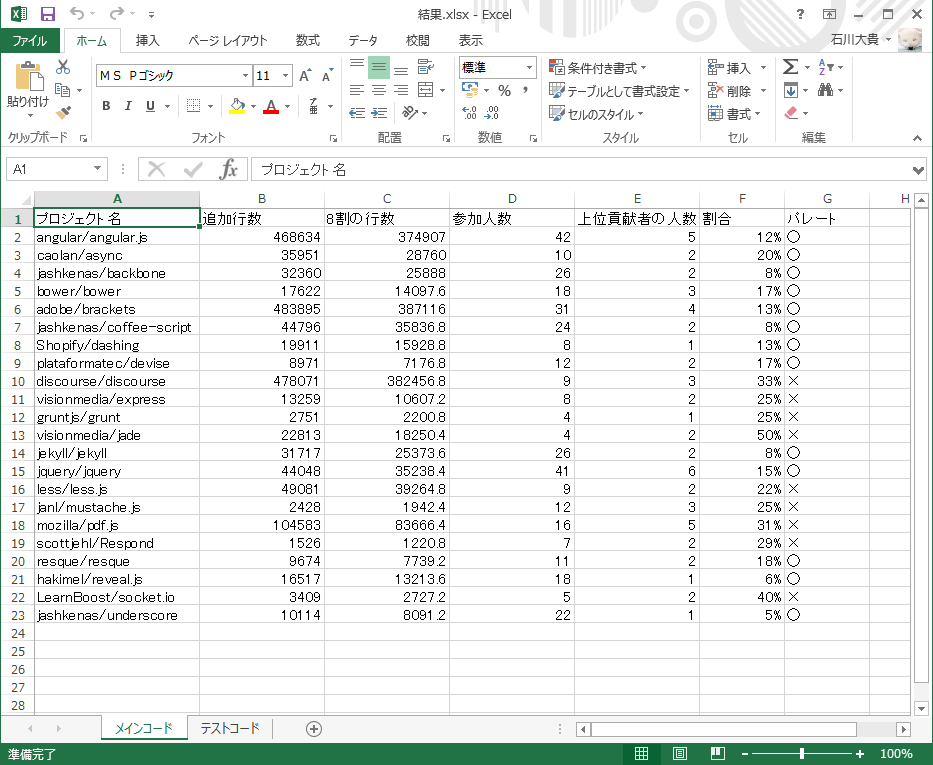
\includegraphics[width=13cm]{matome1.png}
\caption{メインコードでパレートの法則が成り立つか}
\end{figure}

\newpage

%図の挿入
\begin{figure}[h]
\centering
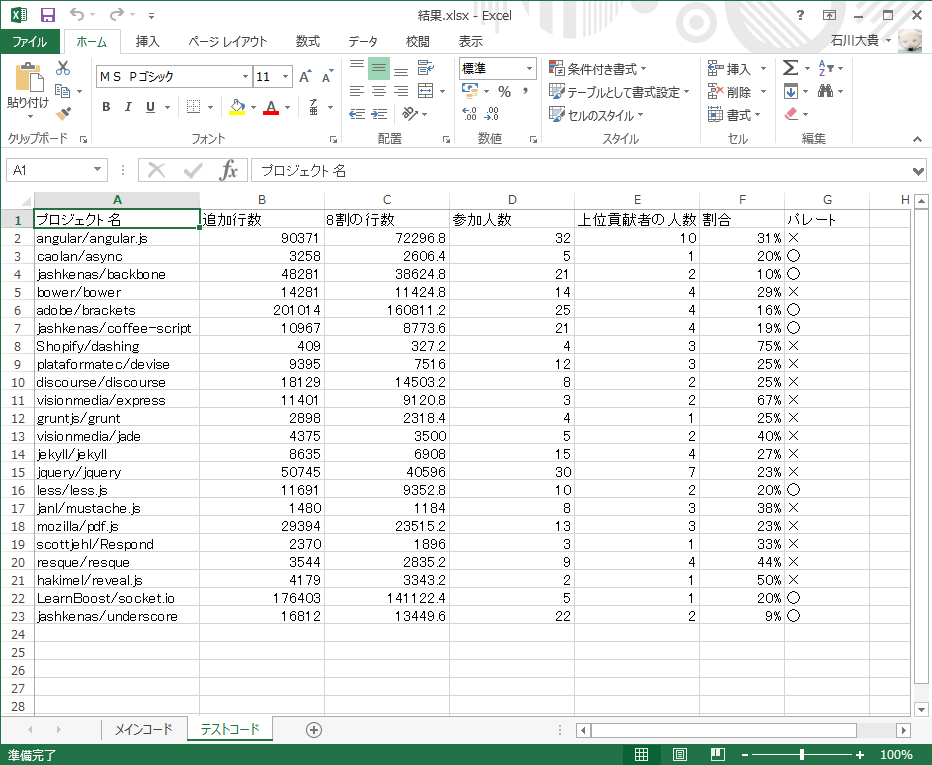
\includegraphics[width=13cm]{matome2.png}
\caption{テストコードでパレートの法則が成り立つか}
\end{figure}

左の列からプロジェクト名,追加行数,8割の行数,参加人数,上位の貢献者の人数,パレートが入力されている.追加行数は,メインコードもしくはテストコードにコミットで追加された,全メンバの合計のコード行数である.8割の行数は,追加行数に0.8を掛けた数で上位の貢献者を探す際の基準にした数値である.参加人数は,メインコードもしくはテストコードで1行以上のコードを追加した人数である.上位の貢献者の人数は,8割の行数をより多く書いていたメンバの人数である.割合は,上位の貢献者の人数÷参加人数をした数値でパレートの法則が成り立つか基準にした数値である.パレートは,パレートの法則が成り立つ場合に○,成り立たない場合に×を入力している.

パレートの法則が成り立つプロジェクトはメインコードでは22件中13件であり,テストコードでは22件中7件であった.

OSS開発でもパレートの法則が成り立つことが考えられるが,同じプロジェクトでもメインコードよりテストコードの方が成り立つ可能性が少ない.これは,メインコードもテストコードも貢献度が高いメンバの人数はあまり変わらないのに対し,メインコードよりテストコードの方が,参加メンバが少ないためだと考える.

また,参加人数が少ないプロジェクトより参加人数が多いプロジェクトの方が,パレートの法則が成り立つことが多いように見える.これは,参加人数が増えることで貢献度の高いメンバと低いメンバの差が大きく開いてくるからだと考える.少数でプロジェクトを進める方がメンバの作業量のばらつきはないようだ.

\newpage

メインコードとテストコードの両方で貢献度の高いメンバに違いがあるのか比べた.メインコードとテストコードの両方で貢献しているメンバがいた場合にその人数を数えた.
まとめた結果を次に記す.

%図の挿入
\begin{figure}[h]
\centering
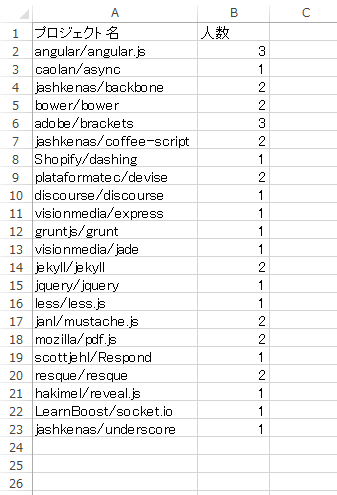
\includegraphics[width=10cm]{matome3.png}
\caption{貢献度の高いメンバの人数}
\end{figure}

\newpage

メインコードとテストコードの両方で貢献しているメンバは1から3人ほどであり,その他はどちらかで貢献していることが多かった.少数のメンバがメインコードとテストコードの両方で貢献度が高く,そのメンバが中心的に活動していると考える.メインコードとテストコードを書いているメンバは同一人物で違いはあまりないと考えていたが,メインコードとテストコードのどちらかだけで貢献するなど,メインコードとテストコードで違いが出た.

このように,メインコードとテストコードごとでメンバによるプロジェクトへの貢献度の違いを見ることができた.



\chapter{結論}

本研究では,GitHub上のプロジェクトを調査することにより,テスト駆動開発において,個人の貢献度がメインコードとテストコードで違いがあるのかを調査した.

主にパレートの法則をもとにし,それぞれのプロジェクトを比較した.OSS開発の現場でもパレートの法則は成り立つ場合がある.メンバによる貢献度の違いが明らかになったため,貢献度の高いメンバの開発手法を参考にすることで,より効率的な開発が可能になると考える.

メインコードとテストコードを書いているメンバは同一人物でない場合が多かった.全体的にテストコードを書くメンバが少ないため,テストコードを書くことでプロジェクトへの貢献度は高まると考える.



\bibliographystyle{junsrt}
\bibliography{biblio}%「biblio.bib」というファイルが必要.



\chapter{謝辞}

本研究を進めるにあたり,矢吹研究室矢吹太朗准教授には,多くの時間をご指導にさいて頂きました.また,矢吹研究室の皆様には,多くの知識や示唆を頂きました.協力していただいた皆様に感謝の気持ちと御礼を申し上げます.

\end{document}
